\documentclass[twoside]{book}

% Packages required by doxygen
\usepackage{fixltx2e}
\usepackage{calc}
\usepackage{doxygen}
\usepackage[export]{adjustbox} % also loads graphicx
\usepackage{graphicx}
\usepackage[utf8]{inputenc}
\usepackage{makeidx}
\usepackage{multicol}
\usepackage{multirow}
\PassOptionsToPackage{warn}{textcomp}
\usepackage{textcomp}
\usepackage[nointegrals]{wasysym}
\usepackage[table]{xcolor}

% Font selection
\usepackage[T1]{fontenc}
\usepackage[scaled=.90]{helvet}
\usepackage{courier}
\usepackage{amssymb}
\usepackage{sectsty}
\renewcommand{\familydefault}{\sfdefault}
\allsectionsfont{%
  \fontseries{bc}\selectfont%
  \color{darkgray}%
}
\renewcommand{\DoxyLabelFont}{%
  \fontseries{bc}\selectfont%
  \color{darkgray}%
}
\newcommand{\+}{\discretionary{\mbox{\scriptsize$\hookleftarrow$}}{}{}}

% Page & text layout
\usepackage{geometry}
\geometry{%
  a4paper,%
  top=2.5cm,%
  bottom=2.5cm,%
  left=2.5cm,%
  right=2.5cm%
}
\tolerance=750
\hfuzz=15pt
\hbadness=750
\setlength{\emergencystretch}{15pt}
\setlength{\parindent}{0cm}
\setlength{\parskip}{3ex plus 2ex minus 2ex}
\makeatletter
\renewcommand{\paragraph}{%
  \@startsection{paragraph}{4}{0ex}{-1.0ex}{1.0ex}{%
    \normalfont\normalsize\bfseries\SS@parafont%
  }%
}
\renewcommand{\subparagraph}{%
  \@startsection{subparagraph}{5}{0ex}{-1.0ex}{1.0ex}{%
    \normalfont\normalsize\bfseries\SS@subparafont%
  }%
}
\makeatother

% Headers & footers
\usepackage{fancyhdr}
\pagestyle{fancyplain}
\fancyhead[LE]{\fancyplain{}{\bfseries\thepage}}
\fancyhead[CE]{\fancyplain{}{}}
\fancyhead[RE]{\fancyplain{}{\bfseries\leftmark}}
\fancyhead[LO]{\fancyplain{}{\bfseries\rightmark}}
\fancyhead[CO]{\fancyplain{}{}}
\fancyhead[RO]{\fancyplain{}{\bfseries\thepage}}
\fancyfoot[LE]{\fancyplain{}{}}
\fancyfoot[CE]{\fancyplain{}{}}
\fancyfoot[RE]{\fancyplain{}{\bfseries\scriptsize Generated by Doxygen }}
\fancyfoot[LO]{\fancyplain{}{\bfseries\scriptsize Generated by Doxygen }}
\fancyfoot[CO]{\fancyplain{}{}}
\fancyfoot[RO]{\fancyplain{}{}}
\renewcommand{\footrulewidth}{0.4pt}
\renewcommand{\chaptermark}[1]{%
  \markboth{#1}{}%
}
\renewcommand{\sectionmark}[1]{%
  \markright{\thesection\ #1}%
}

% Indices & bibliography
\usepackage{natbib}
\usepackage[titles]{tocloft}
\setcounter{tocdepth}{3}
\setcounter{secnumdepth}{5}
\makeindex

% Hyperlinks (required, but should be loaded last)
\usepackage{ifpdf}
\ifpdf
  \usepackage[pdftex,pagebackref=true]{hyperref}
\else
  \usepackage[ps2pdf,pagebackref=true]{hyperref}
\fi
\hypersetup{%
  colorlinks=true,%
  linkcolor=blue,%
  citecolor=blue,%
  unicode%
}

% Custom commands
\newcommand{\clearemptydoublepage}{%
  \newpage{\pagestyle{empty}\cleardoublepage}%
}

\usepackage{caption}
\captionsetup{labelsep=space,justification=centering,font={bf},singlelinecheck=off,skip=4pt,position=top}

%===== C O N T E N T S =====

\begin{document}

% Titlepage & ToC
\hypersetup{pageanchor=false,
             bookmarksnumbered=true,
             pdfencoding=unicode
            }
\pagenumbering{alph}
\begin{titlepage}
\vspace*{7cm}
\begin{center}%
{\Large Money\+Money\+Perf }\\
\vspace*{1cm}
{\large Generated by Doxygen 1.8.14}\\
\end{center}
\end{titlepage}
\clearemptydoublepage
\pagenumbering{roman}
\tableofcontents
\clearemptydoublepage
\pagenumbering{arabic}
\hypersetup{pageanchor=true}

%--- Begin generated contents ---
\chapter{Namespace Index}
\section{Packages}
Here are the packages with brief descriptions (if available)\+:\begin{DoxyCompactList}
\item\contentsline{section}{\mbox{\hyperlink{namespacees}{es}} }{\pageref{namespacees}}{}
\item\contentsline{section}{\mbox{\hyperlink{namespacees_1_1deusto}{es.\+deusto}} }{\pageref{namespacees_1_1deusto}}{}
\item\contentsline{section}{\mbox{\hyperlink{namespacees_1_1deusto_1_1testing}{es.\+deusto.\+testing}} }{\pageref{namespacees_1_1deusto_1_1testing}}{}
\item\contentsline{section}{\mbox{\hyperlink{namespacees_1_1deusto_1_1testing_1_1junit}{es.\+deusto.\+testing.\+junit}} \\*This is the brief documentation for the Java package \mbox{\hyperlink{namespacees_1_1deusto_1_1testing_1_1junit}{es.\+deusto.\+testing.\+junit}} intended for testing Doxygen. May 12, 2014 }{\pageref{namespacees_1_1deusto_1_1testing_1_1junit}}{}
\end{DoxyCompactList}

\chapter{Hierarchical Index}
\section{Class Hierarchy}
This inheritance list is sorted roughly, but not completely, alphabetically\+:\begin{DoxyCompactList}
\item \contentsline{section}{es.\+deusto.\+testing.\+junit.\+I\+Money}{\pageref{interfacees_1_1deusto_1_1testing_1_1junit_1_1_i_money}}{}
\begin{DoxyCompactList}
\item \contentsline{section}{es.\+deusto.\+testing.\+junit.\+Money}{\pageref{classes_1_1deusto_1_1testing_1_1junit_1_1_money}}{}
\item \contentsline{section}{es.\+deusto.\+testing.\+junit.\+Money\+Bag}{\pageref{classes_1_1deusto_1_1testing_1_1junit_1_1_money_bag}}{}
\end{DoxyCompactList}
\end{DoxyCompactList}

\chapter{Class Index}
\section{Class List}
Here are the classes, structs, unions and interfaces with brief descriptions\+:\begin{DoxyCompactList}
\item\contentsline{section}{\mbox{\hyperlink{interfacees_1_1deusto_1_1testing_1_1junit_1_1_i_money}{es.\+deusto.\+testing.\+junit.\+I\+Money}} }{\pageref{interfacees_1_1deusto_1_1testing_1_1junit_1_1_i_money}}{}
\item\contentsline{section}{\mbox{\hyperlink{classes_1_1deusto_1_1testing_1_1junit_1_1_money}{es.\+deusto.\+testing.\+junit.\+Money}} }{\pageref{classes_1_1deusto_1_1testing_1_1junit_1_1_money}}{}
\item\contentsline{section}{\mbox{\hyperlink{classes_1_1deusto_1_1testing_1_1junit_1_1_money_bag}{es.\+deusto.\+testing.\+junit.\+Money\+Bag}} }{\pageref{classes_1_1deusto_1_1testing_1_1junit_1_1_money_bag}}{}
\end{DoxyCompactList}

\chapter{File Index}
\section{File List}
Here is a list of all files with brief descriptions\+:\begin{DoxyCompactList}
\item\contentsline{section}{src/main/java/es/deusto/testing/junit/\mbox{\hyperlink{_i_money_8java}{I\+Money.\+java}} }{\pageref{_i_money_8java}}{}
\item\contentsline{section}{src/main/java/es/deusto/testing/junit/\mbox{\hyperlink{_money_8java}{Money.\+java}} }{\pageref{_money_8java}}{}
\item\contentsline{section}{src/main/java/es/deusto/testing/junit/\mbox{\hyperlink{_money_bag_8java}{Money\+Bag.\+java}} }{\pageref{_money_bag_8java}}{}
\end{DoxyCompactList}

\chapter{Namespace Documentation}
\hypertarget{namespacees}{}\section{Package es}
\label{namespacees}\index{es@{es}}
\subsection*{Packages}
\begin{DoxyCompactItemize}
\item 
package \mbox{\hyperlink{namespacees_1_1deusto}{deusto}}
\end{DoxyCompactItemize}

\hypertarget{namespacees_1_1deusto}{}\section{Package es.\+deusto}
\label{namespacees_1_1deusto}\index{es.\+deusto@{es.\+deusto}}
\subsection*{Packages}
\begin{DoxyCompactItemize}
\item 
package \mbox{\hyperlink{namespacees_1_1deusto_1_1testing}{testing}}
\end{DoxyCompactItemize}

\hypertarget{namespacees_1_1deusto_1_1testing}{}\section{Package es.\+deusto.\+testing}
\label{namespacees_1_1deusto_1_1testing}\index{es.\+deusto.\+testing@{es.\+deusto.\+testing}}
\subsection*{Packages}
\begin{DoxyCompactItemize}
\item 
package \mbox{\hyperlink{namespacees_1_1deusto_1_1testing_1_1junit}{junit}}
\begin{DoxyCompactList}\small\item\em This is the brief documentation for the Java package \mbox{\hyperlink{namespacees_1_1deusto_1_1testing_1_1junit}{es.\+deusto.\+testing.\+junit}} intended for testing Doxygen. May 12, 2014. \end{DoxyCompactList}\end{DoxyCompactItemize}

\hypertarget{namespacees_1_1deusto_1_1testing_1_1junit}{}\section{Package es.\+deusto.\+testing.\+junit}
\label{namespacees_1_1deusto_1_1testing_1_1junit}\index{es.\+deusto.\+testing.\+junit@{es.\+deusto.\+testing.\+junit}}


This is the brief documentation for the Java package \mbox{\hyperlink{namespacees_1_1deusto_1_1testing_1_1junit}{es.\+deusto.\+testing.\+junit}} intended for testing Doxygen. May 12, 2014.  


\subsection*{Classes}
\begin{DoxyCompactItemize}
\item 
interface \mbox{\hyperlink{interfacees_1_1deusto_1_1testing_1_1junit_1_1_i_money}{I\+Money}}
\item 
class \mbox{\hyperlink{classes_1_1deusto_1_1testing_1_1junit_1_1_money}{Money}}
\item 
class \mbox{\hyperlink{classes_1_1deusto_1_1testing_1_1junit_1_1_money_bag}{Money\+Bag}}
\end{DoxyCompactItemize}


\subsection{Detailed Description}
This is the brief documentation for the Java package \mbox{\hyperlink{namespacees_1_1deusto_1_1testing_1_1junit}{es.\+deusto.\+testing.\+junit}} intended for testing Doxygen. May 12, 2014. 

This is the detailed description of a package composed by classes \mbox{\hyperlink{classes_1_1deusto_1_1testing_1_1junit_1_1_money}{Money}} and \mbox{\hyperlink{classes_1_1deusto_1_1testing_1_1junit_1_1_money_bag}{Money\+Bag}} which inherit from \mbox{\hyperlink{interfacees_1_1deusto_1_1testing_1_1junit_1_1_i_money}{I\+Money}} and are tested in class Money\+Perf\+Test 
\chapter{Class Documentation}
\hypertarget{interfacees_1_1deusto_1_1testing_1_1junit_1_1_i_money}{}\section{es.\+deusto.\+testing.\+junit.\+I\+Money Interface Reference}
\label{interfacees_1_1deusto_1_1testing_1_1junit_1_1_i_money}\index{es.\+deusto.\+testing.\+junit.\+I\+Money@{es.\+deusto.\+testing.\+junit.\+I\+Money}}


Inheritance diagram for es.\+deusto.\+testing.\+junit.\+I\+Money\+:\nopagebreak
\begin{figure}[H]
\begin{center}
\leavevmode
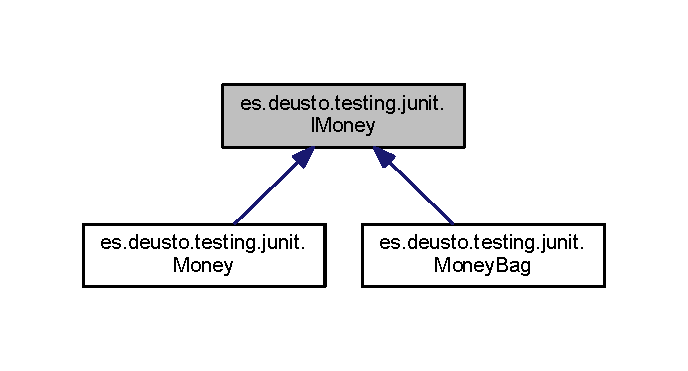
\includegraphics[width=330pt]{interfacees_1_1deusto_1_1testing_1_1junit_1_1_i_money__inherit__graph}
\end{center}
\end{figure}
\subsection*{Public Member Functions}
\begin{DoxyCompactItemize}
\item 
abstract \mbox{\hyperlink{interfacees_1_1deusto_1_1testing_1_1junit_1_1_i_money}{I\+Money}} \mbox{\hyperlink{interfacees_1_1deusto_1_1testing_1_1junit_1_1_i_money_a7f3ac1ced239e64294706155c569b8de}{add}} (\mbox{\hyperlink{interfacees_1_1deusto_1_1testing_1_1junit_1_1_i_money}{I\+Money}} m)
\item 
abstract \mbox{\hyperlink{interfacees_1_1deusto_1_1testing_1_1junit_1_1_i_money}{I\+Money}} \mbox{\hyperlink{interfacees_1_1deusto_1_1testing_1_1junit_1_1_i_money_aab8d4be667a542a8aa1380eb2b6e4257}{add\+Money}} (\mbox{\hyperlink{classes_1_1deusto_1_1testing_1_1junit_1_1_money}{Money}} m)
\item 
abstract \mbox{\hyperlink{interfacees_1_1deusto_1_1testing_1_1junit_1_1_i_money}{I\+Money}} \mbox{\hyperlink{interfacees_1_1deusto_1_1testing_1_1junit_1_1_i_money_ac47c8940f0565bd9eda16730170bc9f7}{add\+Money\+Bag}} (\mbox{\hyperlink{classes_1_1deusto_1_1testing_1_1junit_1_1_money_bag}{Money\+Bag}} s)
\item 
abstract boolean \mbox{\hyperlink{interfacees_1_1deusto_1_1testing_1_1junit_1_1_i_money_a166c39b6f931e49769580a04f8c73500}{is\+Zero}} ()
\item 
abstract \mbox{\hyperlink{interfacees_1_1deusto_1_1testing_1_1junit_1_1_i_money}{I\+Money}} \mbox{\hyperlink{interfacees_1_1deusto_1_1testing_1_1junit_1_1_i_money_a09154f9713133d4734f72d6a20081209}{multiply}} (int factor)
\item 
abstract \mbox{\hyperlink{interfacees_1_1deusto_1_1testing_1_1junit_1_1_i_money}{I\+Money}} \mbox{\hyperlink{interfacees_1_1deusto_1_1testing_1_1junit_1_1_i_money_a741967d7aa89055b6873619303b11385}{negate}} ()
\item 
abstract \mbox{\hyperlink{interfacees_1_1deusto_1_1testing_1_1junit_1_1_i_money}{I\+Money}} \mbox{\hyperlink{interfacees_1_1deusto_1_1testing_1_1junit_1_1_i_money_a1fb4981aa759e3fe0679654bec7a8b61}{subtract}} (\mbox{\hyperlink{interfacees_1_1deusto_1_1testing_1_1junit_1_1_i_money}{I\+Money}} m)
\item 
abstract void \mbox{\hyperlink{interfacees_1_1deusto_1_1testing_1_1junit_1_1_i_money_ae45bc758e69a0017f083f11d050c53cb}{append\+To}} (\mbox{\hyperlink{classes_1_1deusto_1_1testing_1_1junit_1_1_money_bag}{Money\+Bag}} m)
\begin{DoxyCompactList}\small\item\em Brief test for \mbox{\hyperlink{interfacees_1_1deusto_1_1testing_1_1junit_1_1_i_money_ae45bc758e69a0017f083f11d050c53cb}{append\+To()}} added May 12, 2014. \end{DoxyCompactList}\end{DoxyCompactItemize}


\subsection{Detailed Description}


Definition at line 3 of file I\+Money.\+java.



\subsection{Member Function Documentation}
\mbox{\Hypertarget{interfacees_1_1deusto_1_1testing_1_1junit_1_1_i_money_a7f3ac1ced239e64294706155c569b8de}\label{interfacees_1_1deusto_1_1testing_1_1junit_1_1_i_money_a7f3ac1ced239e64294706155c569b8de}} 
\index{es\+::deusto\+::testing\+::junit\+::\+I\+Money@{es\+::deusto\+::testing\+::junit\+::\+I\+Money}!add@{add}}
\index{add@{add}!es\+::deusto\+::testing\+::junit\+::\+I\+Money@{es\+::deusto\+::testing\+::junit\+::\+I\+Money}}
\subsubsection{\texorpdfstring{add()}{add()}}
{\footnotesize\ttfamily abstract \mbox{\hyperlink{interfacees_1_1deusto_1_1testing_1_1junit_1_1_i_money}{I\+Money}} es.\+deusto.\+testing.\+junit.\+I\+Money.\+add (\begin{DoxyParamCaption}\item[{\mbox{\hyperlink{interfacees_1_1deusto_1_1testing_1_1junit_1_1_i_money}{I\+Money}}}]{m }\end{DoxyParamCaption})\hspace{0.3cm}{\ttfamily [abstract]}}

Adds a money to this money. 

Implemented in \mbox{\hyperlink{classes_1_1deusto_1_1testing_1_1junit_1_1_money_bag_ab3be83ff12fa6d19b67b669194120d00}{es.\+deusto.\+testing.\+junit.\+Money\+Bag}}, and \mbox{\hyperlink{classes_1_1deusto_1_1testing_1_1junit_1_1_money_a6a3d64861c49dee89ffd0ed0c576045d}{es.\+deusto.\+testing.\+junit.\+Money}}.

\mbox{\Hypertarget{interfacees_1_1deusto_1_1testing_1_1junit_1_1_i_money_aab8d4be667a542a8aa1380eb2b6e4257}\label{interfacees_1_1deusto_1_1testing_1_1junit_1_1_i_money_aab8d4be667a542a8aa1380eb2b6e4257}} 
\index{es\+::deusto\+::testing\+::junit\+::\+I\+Money@{es\+::deusto\+::testing\+::junit\+::\+I\+Money}!add\+Money@{add\+Money}}
\index{add\+Money@{add\+Money}!es\+::deusto\+::testing\+::junit\+::\+I\+Money@{es\+::deusto\+::testing\+::junit\+::\+I\+Money}}
\subsubsection{\texorpdfstring{add\+Money()}{addMoney()}}
{\footnotesize\ttfamily abstract \mbox{\hyperlink{interfacees_1_1deusto_1_1testing_1_1junit_1_1_i_money}{I\+Money}} es.\+deusto.\+testing.\+junit.\+I\+Money.\+add\+Money (\begin{DoxyParamCaption}\item[{\mbox{\hyperlink{classes_1_1deusto_1_1testing_1_1junit_1_1_money}{Money}}}]{m }\end{DoxyParamCaption})\hspace{0.3cm}{\ttfamily [abstract]}}

Adds a simple \mbox{\hyperlink{classes_1_1deusto_1_1testing_1_1junit_1_1_money}{Money}} to this money. This is a helper method for implementing double dispatch 

Implemented in \mbox{\hyperlink{classes_1_1deusto_1_1testing_1_1junit_1_1_money_bag_a06ecedbf53ba09d34276fe177e3169bc}{es.\+deusto.\+testing.\+junit.\+Money\+Bag}}, and \mbox{\hyperlink{classes_1_1deusto_1_1testing_1_1junit_1_1_money_a223a447d5daf23b5e9cc0f551b72e328}{es.\+deusto.\+testing.\+junit.\+Money}}.

Here is the caller graph for this function\+:\nopagebreak
\begin{figure}[H]
\begin{center}
\leavevmode
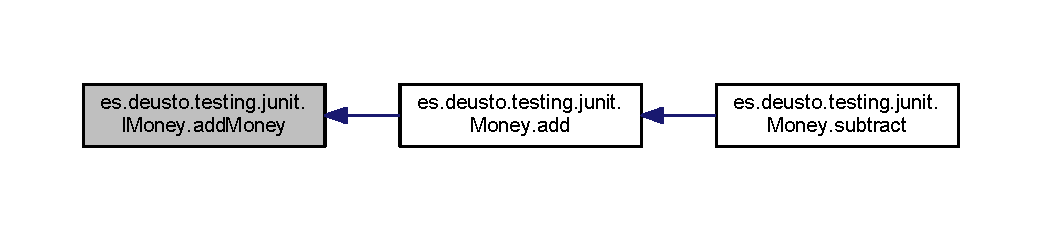
\includegraphics[width=350pt]{interfacees_1_1deusto_1_1testing_1_1junit_1_1_i_money_aab8d4be667a542a8aa1380eb2b6e4257_icgraph}
\end{center}
\end{figure}
\mbox{\Hypertarget{interfacees_1_1deusto_1_1testing_1_1junit_1_1_i_money_ac47c8940f0565bd9eda16730170bc9f7}\label{interfacees_1_1deusto_1_1testing_1_1junit_1_1_i_money_ac47c8940f0565bd9eda16730170bc9f7}} 
\index{es\+::deusto\+::testing\+::junit\+::\+I\+Money@{es\+::deusto\+::testing\+::junit\+::\+I\+Money}!add\+Money\+Bag@{add\+Money\+Bag}}
\index{add\+Money\+Bag@{add\+Money\+Bag}!es\+::deusto\+::testing\+::junit\+::\+I\+Money@{es\+::deusto\+::testing\+::junit\+::\+I\+Money}}
\subsubsection{\texorpdfstring{add\+Money\+Bag()}{addMoneyBag()}}
{\footnotesize\ttfamily abstract \mbox{\hyperlink{interfacees_1_1deusto_1_1testing_1_1junit_1_1_i_money}{I\+Money}} es.\+deusto.\+testing.\+junit.\+I\+Money.\+add\+Money\+Bag (\begin{DoxyParamCaption}\item[{\mbox{\hyperlink{classes_1_1deusto_1_1testing_1_1junit_1_1_money_bag}{Money\+Bag}}}]{s }\end{DoxyParamCaption})\hspace{0.3cm}{\ttfamily [abstract]}}

Adds a \mbox{\hyperlink{classes_1_1deusto_1_1testing_1_1junit_1_1_money_bag}{Money\+Bag}} to this money. This is a helper method for implementing double dispatch 

Implemented in \mbox{\hyperlink{classes_1_1deusto_1_1testing_1_1junit_1_1_money_bag_ab329e6a2811b83a2b1670b79be92249d}{es.\+deusto.\+testing.\+junit.\+Money\+Bag}}, and \mbox{\hyperlink{classes_1_1deusto_1_1testing_1_1junit_1_1_money_ad9a107a6884026a1bb12102d3a8a5b41}{es.\+deusto.\+testing.\+junit.\+Money}}.

Here is the caller graph for this function\+:\nopagebreak
\begin{figure}[H]
\begin{center}
\leavevmode
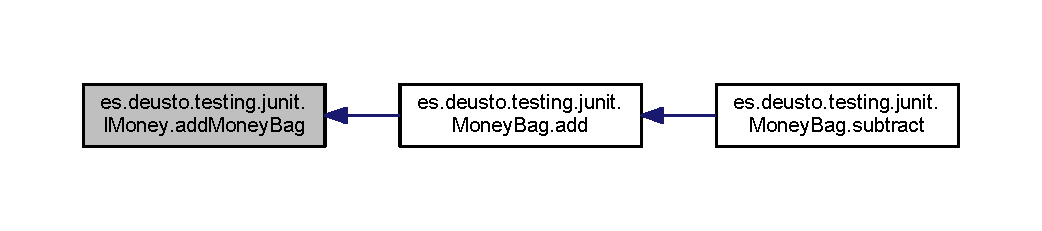
\includegraphics[width=350pt]{interfacees_1_1deusto_1_1testing_1_1junit_1_1_i_money_ac47c8940f0565bd9eda16730170bc9f7_icgraph}
\end{center}
\end{figure}
\mbox{\Hypertarget{interfacees_1_1deusto_1_1testing_1_1junit_1_1_i_money_ae45bc758e69a0017f083f11d050c53cb}\label{interfacees_1_1deusto_1_1testing_1_1junit_1_1_i_money_ae45bc758e69a0017f083f11d050c53cb}} 
\index{es\+::deusto\+::testing\+::junit\+::\+I\+Money@{es\+::deusto\+::testing\+::junit\+::\+I\+Money}!append\+To@{append\+To}}
\index{append\+To@{append\+To}!es\+::deusto\+::testing\+::junit\+::\+I\+Money@{es\+::deusto\+::testing\+::junit\+::\+I\+Money}}
\subsubsection{\texorpdfstring{append\+To()}{appendTo()}}
{\footnotesize\ttfamily abstract void es.\+deusto.\+testing.\+junit.\+I\+Money.\+append\+To (\begin{DoxyParamCaption}\item[{\mbox{\hyperlink{classes_1_1deusto_1_1testing_1_1junit_1_1_money_bag}{Money\+Bag}}}]{m }\end{DoxyParamCaption})\hspace{0.3cm}{\ttfamily [abstract]}}



Brief test for \mbox{\hyperlink{interfacees_1_1deusto_1_1testing_1_1junit_1_1_i_money_ae45bc758e69a0017f083f11d050c53cb}{append\+To()}} added May 12, 2014. 

Append this to a \mbox{\hyperlink{classes_1_1deusto_1_1testing_1_1junit_1_1_money_bag}{Money\+Bag}} m. \mbox{\hyperlink{interfacees_1_1deusto_1_1testing_1_1junit_1_1_i_money_ae45bc758e69a0017f083f11d050c53cb}{append\+To()}} needs to be public because it is used polymorphically, but it should not be used by clients because it modifies the argument m. 

Implemented in \mbox{\hyperlink{classes_1_1deusto_1_1testing_1_1junit_1_1_money_bag_ac8a5877b35b12939ce14543872ed18af}{es.\+deusto.\+testing.\+junit.\+Money\+Bag}}, and \mbox{\hyperlink{classes_1_1deusto_1_1testing_1_1junit_1_1_money_aa9a6df9f35118060914ae6e8f74d1d51}{es.\+deusto.\+testing.\+junit.\+Money}}.

Here is the caller graph for this function\+:\nopagebreak
\begin{figure}[H]
\begin{center}
\leavevmode
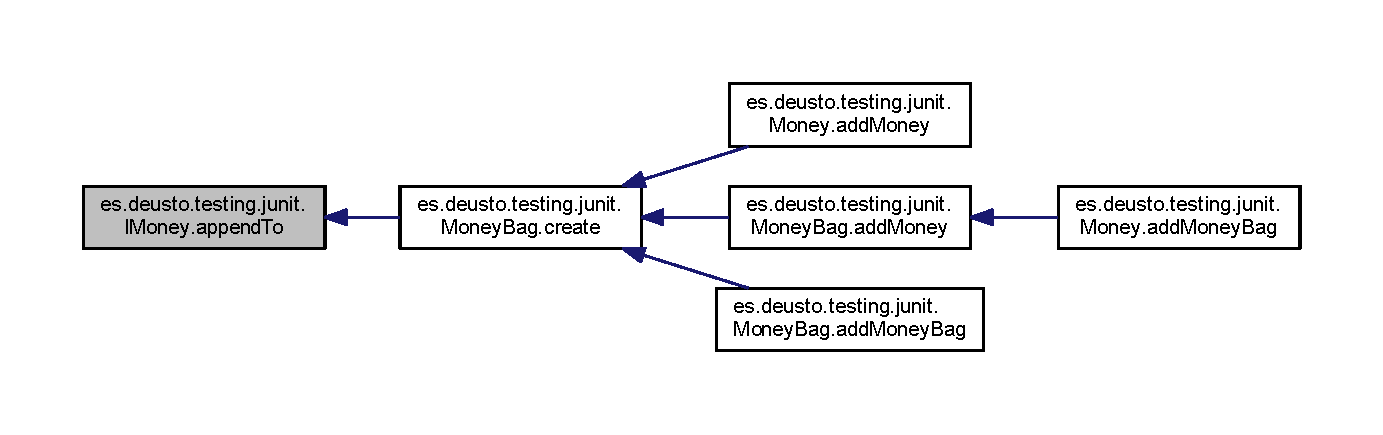
\includegraphics[width=350pt]{interfacees_1_1deusto_1_1testing_1_1junit_1_1_i_money_ae45bc758e69a0017f083f11d050c53cb_icgraph}
\end{center}
\end{figure}
\mbox{\Hypertarget{interfacees_1_1deusto_1_1testing_1_1junit_1_1_i_money_a166c39b6f931e49769580a04f8c73500}\label{interfacees_1_1deusto_1_1testing_1_1junit_1_1_i_money_a166c39b6f931e49769580a04f8c73500}} 
\index{es\+::deusto\+::testing\+::junit\+::\+I\+Money@{es\+::deusto\+::testing\+::junit\+::\+I\+Money}!is\+Zero@{is\+Zero}}
\index{is\+Zero@{is\+Zero}!es\+::deusto\+::testing\+::junit\+::\+I\+Money@{es\+::deusto\+::testing\+::junit\+::\+I\+Money}}
\subsubsection{\texorpdfstring{is\+Zero()}{isZero()}}
{\footnotesize\ttfamily abstract boolean es.\+deusto.\+testing.\+junit.\+I\+Money.\+is\+Zero (\begin{DoxyParamCaption}{ }\end{DoxyParamCaption})\hspace{0.3cm}{\ttfamily [abstract]}}

Tests whether this money is zero 

Implemented in \mbox{\hyperlink{classes_1_1deusto_1_1testing_1_1junit_1_1_money_bag_abebc5bc39c3343cb3c4e5fb291fd5893}{es.\+deusto.\+testing.\+junit.\+Money\+Bag}}, and \mbox{\hyperlink{classes_1_1deusto_1_1testing_1_1junit_1_1_money_a797658a03260b535e9a36ebbcc3b19c9}{es.\+deusto.\+testing.\+junit.\+Money}}.

\mbox{\Hypertarget{interfacees_1_1deusto_1_1testing_1_1junit_1_1_i_money_a09154f9713133d4734f72d6a20081209}\label{interfacees_1_1deusto_1_1testing_1_1junit_1_1_i_money_a09154f9713133d4734f72d6a20081209}} 
\index{es\+::deusto\+::testing\+::junit\+::\+I\+Money@{es\+::deusto\+::testing\+::junit\+::\+I\+Money}!multiply@{multiply}}
\index{multiply@{multiply}!es\+::deusto\+::testing\+::junit\+::\+I\+Money@{es\+::deusto\+::testing\+::junit\+::\+I\+Money}}
\subsubsection{\texorpdfstring{multiply()}{multiply()}}
{\footnotesize\ttfamily abstract \mbox{\hyperlink{interfacees_1_1deusto_1_1testing_1_1junit_1_1_i_money}{I\+Money}} es.\+deusto.\+testing.\+junit.\+I\+Money.\+multiply (\begin{DoxyParamCaption}\item[{int}]{factor }\end{DoxyParamCaption})\hspace{0.3cm}{\ttfamily [abstract]}}

Multiplies a money by the given factor. 

Implemented in \mbox{\hyperlink{classes_1_1deusto_1_1testing_1_1junit_1_1_money_bag_aa20ce4cc70c2ba0bc9a5ccb96635d506}{es.\+deusto.\+testing.\+junit.\+Money\+Bag}}, and \mbox{\hyperlink{classes_1_1deusto_1_1testing_1_1junit_1_1_money_a02c7d4e9013710f70d1d46e9c9ebae88}{es.\+deusto.\+testing.\+junit.\+Money}}.

\mbox{\Hypertarget{interfacees_1_1deusto_1_1testing_1_1junit_1_1_i_money_a741967d7aa89055b6873619303b11385}\label{interfacees_1_1deusto_1_1testing_1_1junit_1_1_i_money_a741967d7aa89055b6873619303b11385}} 
\index{es\+::deusto\+::testing\+::junit\+::\+I\+Money@{es\+::deusto\+::testing\+::junit\+::\+I\+Money}!negate@{negate}}
\index{negate@{negate}!es\+::deusto\+::testing\+::junit\+::\+I\+Money@{es\+::deusto\+::testing\+::junit\+::\+I\+Money}}
\subsubsection{\texorpdfstring{negate()}{negate()}}
{\footnotesize\ttfamily abstract \mbox{\hyperlink{interfacees_1_1deusto_1_1testing_1_1junit_1_1_i_money}{I\+Money}} es.\+deusto.\+testing.\+junit.\+I\+Money.\+negate (\begin{DoxyParamCaption}{ }\end{DoxyParamCaption})\hspace{0.3cm}{\ttfamily [abstract]}}

Negates this money. 

Implemented in \mbox{\hyperlink{classes_1_1deusto_1_1testing_1_1junit_1_1_money_bag_abf06bf97e548f95038756608fe0c8351}{es.\+deusto.\+testing.\+junit.\+Money\+Bag}}, and \mbox{\hyperlink{classes_1_1deusto_1_1testing_1_1junit_1_1_money_ae5f0bc3ea87f1fd55d6478653b8f2e36}{es.\+deusto.\+testing.\+junit.\+Money}}.

Here is the caller graph for this function\+:\nopagebreak
\begin{figure}[H]
\begin{center}
\leavevmode
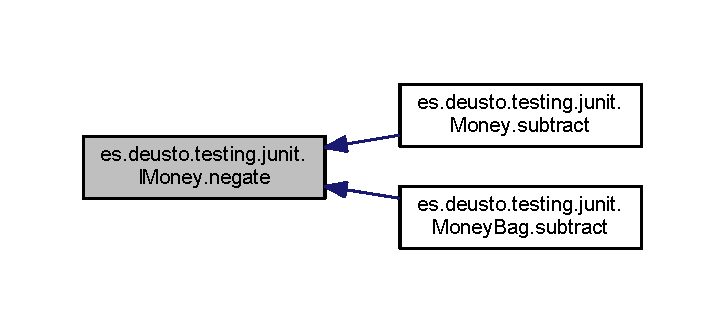
\includegraphics[width=348pt]{interfacees_1_1deusto_1_1testing_1_1junit_1_1_i_money_a741967d7aa89055b6873619303b11385_icgraph}
\end{center}
\end{figure}
\mbox{\Hypertarget{interfacees_1_1deusto_1_1testing_1_1junit_1_1_i_money_a1fb4981aa759e3fe0679654bec7a8b61}\label{interfacees_1_1deusto_1_1testing_1_1junit_1_1_i_money_a1fb4981aa759e3fe0679654bec7a8b61}} 
\index{es\+::deusto\+::testing\+::junit\+::\+I\+Money@{es\+::deusto\+::testing\+::junit\+::\+I\+Money}!subtract@{subtract}}
\index{subtract@{subtract}!es\+::deusto\+::testing\+::junit\+::\+I\+Money@{es\+::deusto\+::testing\+::junit\+::\+I\+Money}}
\subsubsection{\texorpdfstring{subtract()}{subtract()}}
{\footnotesize\ttfamily abstract \mbox{\hyperlink{interfacees_1_1deusto_1_1testing_1_1junit_1_1_i_money}{I\+Money}} es.\+deusto.\+testing.\+junit.\+I\+Money.\+subtract (\begin{DoxyParamCaption}\item[{\mbox{\hyperlink{interfacees_1_1deusto_1_1testing_1_1junit_1_1_i_money}{I\+Money}}}]{m }\end{DoxyParamCaption})\hspace{0.3cm}{\ttfamily [abstract]}}

Subtracts a money from this money. 

Implemented in \mbox{\hyperlink{classes_1_1deusto_1_1testing_1_1junit_1_1_money_bag_a7f1803fe267edca895cdf752b5f46560}{es.\+deusto.\+testing.\+junit.\+Money\+Bag}}, and \mbox{\hyperlink{classes_1_1deusto_1_1testing_1_1junit_1_1_money_aada973cd1a31410ed2b7e5d2ae6bc2e9}{es.\+deusto.\+testing.\+junit.\+Money}}.



The documentation for this interface was generated from the following file\+:\begin{DoxyCompactItemize}
\item 
src/main/java/es/deusto/testing/junit/\mbox{\hyperlink{_i_money_8java}{I\+Money.\+java}}\end{DoxyCompactItemize}

\hypertarget{classes_1_1deusto_1_1testing_1_1junit_1_1_money}{}\section{es.\+deusto.\+testing.\+junit.\+Money Class Reference}
\label{classes_1_1deusto_1_1testing_1_1junit_1_1_money}\index{es.\+deusto.\+testing.\+junit.\+Money@{es.\+deusto.\+testing.\+junit.\+Money}}


Inheritance diagram for es.\+deusto.\+testing.\+junit.\+Money\+:\nopagebreak
\begin{figure}[H]
\begin{center}
\leavevmode
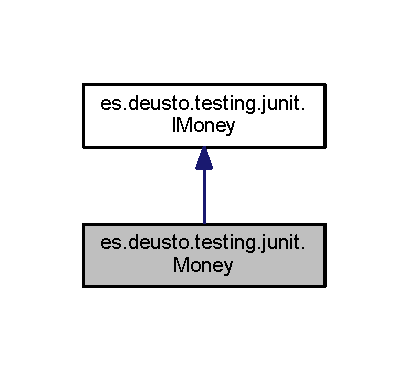
\includegraphics[width=196pt]{classes_1_1deusto_1_1testing_1_1junit_1_1_money__inherit__graph}
\end{center}
\end{figure}


Collaboration diagram for es.\+deusto.\+testing.\+junit.\+Money\+:\nopagebreak
\begin{figure}[H]
\begin{center}
\leavevmode
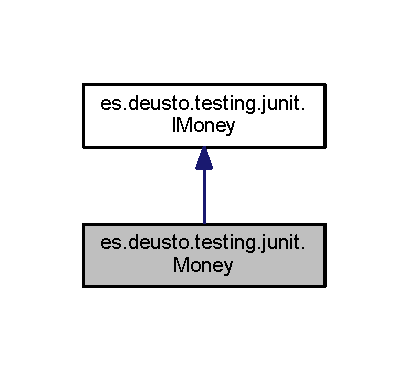
\includegraphics[width=196pt]{classes_1_1deusto_1_1testing_1_1junit_1_1_money__coll__graph}
\end{center}
\end{figure}
\subsection*{Public Member Functions}
\begin{DoxyCompactItemize}
\item 
\mbox{\hyperlink{classes_1_1deusto_1_1testing_1_1junit_1_1_money_a6f1749eb364c59ed038f79cf8965e3bc}{Money}} (int \mbox{\hyperlink{classes_1_1deusto_1_1testing_1_1junit_1_1_money_a9bef5d9027f270e8ce0303e4f929bbd5}{amount}}, String \mbox{\hyperlink{classes_1_1deusto_1_1testing_1_1junit_1_1_money_aefa4aaf62bb653eae25851d98ae02dcb}{currency}})
\item 
\mbox{\hyperlink{interfacees_1_1deusto_1_1testing_1_1junit_1_1_i_money}{I\+Money}} \mbox{\hyperlink{classes_1_1deusto_1_1testing_1_1junit_1_1_money_a6a3d64861c49dee89ffd0ed0c576045d}{add}} (\mbox{\hyperlink{interfacees_1_1deusto_1_1testing_1_1junit_1_1_i_money}{I\+Money}} m)
\item 
\mbox{\hyperlink{interfacees_1_1deusto_1_1testing_1_1junit_1_1_i_money}{I\+Money}} \mbox{\hyperlink{classes_1_1deusto_1_1testing_1_1junit_1_1_money_a223a447d5daf23b5e9cc0f551b72e328}{add\+Money}} (\mbox{\hyperlink{classes_1_1deusto_1_1testing_1_1junit_1_1_money}{Money}} m)
\item 
\mbox{\hyperlink{interfacees_1_1deusto_1_1testing_1_1junit_1_1_i_money}{I\+Money}} \mbox{\hyperlink{classes_1_1deusto_1_1testing_1_1junit_1_1_money_ad9a107a6884026a1bb12102d3a8a5b41}{add\+Money\+Bag}} (\mbox{\hyperlink{classes_1_1deusto_1_1testing_1_1junit_1_1_money_bag}{Money\+Bag}} s)
\item 
int \mbox{\hyperlink{classes_1_1deusto_1_1testing_1_1junit_1_1_money_a9bef5d9027f270e8ce0303e4f929bbd5}{amount}} ()
\item 
String \mbox{\hyperlink{classes_1_1deusto_1_1testing_1_1junit_1_1_money_aefa4aaf62bb653eae25851d98ae02dcb}{currency}} ()
\item 
boolean \mbox{\hyperlink{classes_1_1deusto_1_1testing_1_1junit_1_1_money_a2356df38b8e9ecdd969bab11d6dd301b}{equals}} (Object an\+Object)
\item 
int \mbox{\hyperlink{classes_1_1deusto_1_1testing_1_1junit_1_1_money_af6cfb5b27bf97170d990dea12de04f37}{hash\+Code}} ()
\item 
boolean \mbox{\hyperlink{classes_1_1deusto_1_1testing_1_1junit_1_1_money_a797658a03260b535e9a36ebbcc3b19c9}{is\+Zero}} ()
\item 
\mbox{\hyperlink{interfacees_1_1deusto_1_1testing_1_1junit_1_1_i_money}{I\+Money}} \mbox{\hyperlink{classes_1_1deusto_1_1testing_1_1junit_1_1_money_a02c7d4e9013710f70d1d46e9c9ebae88}{multiply}} (int factor)
\item 
\mbox{\hyperlink{interfacees_1_1deusto_1_1testing_1_1junit_1_1_i_money}{I\+Money}} \mbox{\hyperlink{classes_1_1deusto_1_1testing_1_1junit_1_1_money_ae5f0bc3ea87f1fd55d6478653b8f2e36}{negate}} ()
\item 
\mbox{\hyperlink{interfacees_1_1deusto_1_1testing_1_1junit_1_1_i_money}{I\+Money}} \mbox{\hyperlink{classes_1_1deusto_1_1testing_1_1junit_1_1_money_aada973cd1a31410ed2b7e5d2ae6bc2e9}{subtract}} (\mbox{\hyperlink{interfacees_1_1deusto_1_1testing_1_1junit_1_1_i_money}{I\+Money}} m)
\item 
String \mbox{\hyperlink{classes_1_1deusto_1_1testing_1_1junit_1_1_money_af9e655069123757bea0efecc4efcd638}{to\+String}} ()
\item 
void \mbox{\hyperlink{classes_1_1deusto_1_1testing_1_1junit_1_1_money_aa9a6df9f35118060914ae6e8f74d1d51}{append\+To}} (\mbox{\hyperlink{classes_1_1deusto_1_1testing_1_1junit_1_1_money_bag}{Money\+Bag}} m)
\end{DoxyCompactItemize}


\subsection{Detailed Description}
A simple \mbox{\hyperlink{classes_1_1deusto_1_1testing_1_1junit_1_1_money}{Money}} class. 

Definition at line 12 of file Money.\+java.



\subsection{Constructor \& Destructor Documentation}
\mbox{\Hypertarget{classes_1_1deusto_1_1testing_1_1junit_1_1_money_a6f1749eb364c59ed038f79cf8965e3bc}\label{classes_1_1deusto_1_1testing_1_1junit_1_1_money_a6f1749eb364c59ed038f79cf8965e3bc}} 
\index{es\+::deusto\+::testing\+::junit\+::\+Money@{es\+::deusto\+::testing\+::junit\+::\+Money}!Money@{Money}}
\index{Money@{Money}!es\+::deusto\+::testing\+::junit\+::\+Money@{es\+::deusto\+::testing\+::junit\+::\+Money}}
\subsubsection{\texorpdfstring{Money()}{Money()}}
{\footnotesize\ttfamily es.\+deusto.\+testing.\+junit.\+Money.\+Money (\begin{DoxyParamCaption}\item[{int}]{amount,  }\item[{String}]{currency }\end{DoxyParamCaption})}

Constructs a money from the given amount and currency. 

Definition at line 20 of file Money.\+java.

Here is the call graph for this function\+:\nopagebreak
\begin{figure}[H]
\begin{center}
\leavevmode
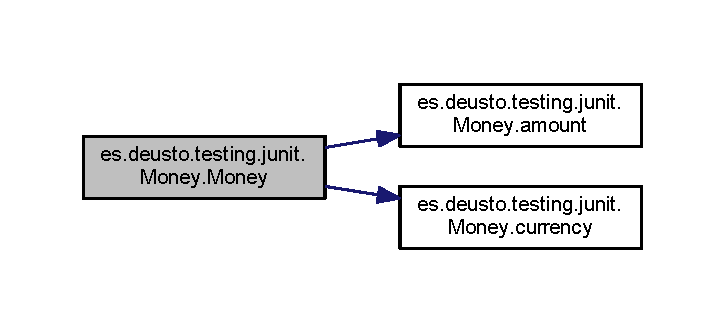
\includegraphics[width=348pt]{classes_1_1deusto_1_1testing_1_1junit_1_1_money_a6f1749eb364c59ed038f79cf8965e3bc_cgraph}
\end{center}
\end{figure}
Here is the caller graph for this function\+:\nopagebreak
\begin{figure}[H]
\begin{center}
\leavevmode
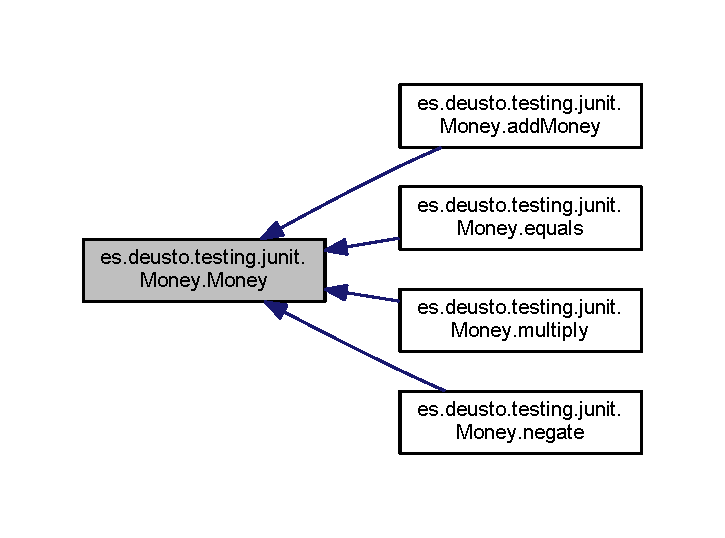
\includegraphics[width=348pt]{classes_1_1deusto_1_1testing_1_1junit_1_1_money_a6f1749eb364c59ed038f79cf8965e3bc_icgraph}
\end{center}
\end{figure}


\subsection{Member Function Documentation}
\mbox{\Hypertarget{classes_1_1deusto_1_1testing_1_1junit_1_1_money_a6a3d64861c49dee89ffd0ed0c576045d}\label{classes_1_1deusto_1_1testing_1_1junit_1_1_money_a6a3d64861c49dee89ffd0ed0c576045d}} 
\index{es\+::deusto\+::testing\+::junit\+::\+Money@{es\+::deusto\+::testing\+::junit\+::\+Money}!add@{add}}
\index{add@{add}!es\+::deusto\+::testing\+::junit\+::\+Money@{es\+::deusto\+::testing\+::junit\+::\+Money}}
\subsubsection{\texorpdfstring{add()}{add()}}
{\footnotesize\ttfamily \mbox{\hyperlink{interfacees_1_1deusto_1_1testing_1_1junit_1_1_i_money}{I\+Money}} es.\+deusto.\+testing.\+junit.\+Money.\+add (\begin{DoxyParamCaption}\item[{\mbox{\hyperlink{interfacees_1_1deusto_1_1testing_1_1junit_1_1_i_money}{I\+Money}}}]{m }\end{DoxyParamCaption})}

Adds a money to this money. Forwards the request to the add\+Money helper. 

Implements \mbox{\hyperlink{interfacees_1_1deusto_1_1testing_1_1junit_1_1_i_money_a7f3ac1ced239e64294706155c569b8de}{es.\+deusto.\+testing.\+junit.\+I\+Money}}.



Definition at line 27 of file Money.\+java.

Here is the call graph for this function\+:\nopagebreak
\begin{figure}[H]
\begin{center}
\leavevmode
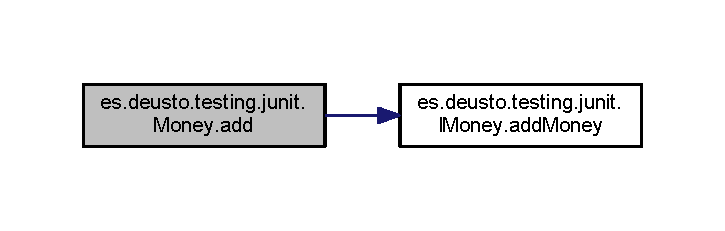
\includegraphics[width=348pt]{classes_1_1deusto_1_1testing_1_1junit_1_1_money_a6a3d64861c49dee89ffd0ed0c576045d_cgraph}
\end{center}
\end{figure}
Here is the caller graph for this function\+:\nopagebreak
\begin{figure}[H]
\begin{center}
\leavevmode
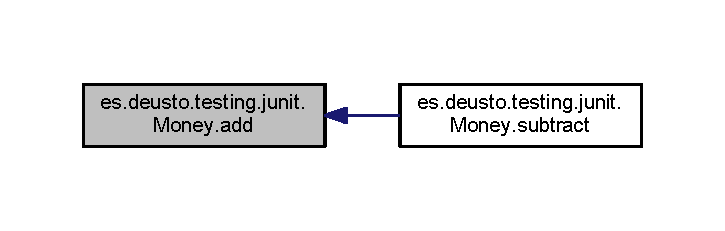
\includegraphics[width=348pt]{classes_1_1deusto_1_1testing_1_1junit_1_1_money_a6a3d64861c49dee89ffd0ed0c576045d_icgraph}
\end{center}
\end{figure}
\mbox{\Hypertarget{classes_1_1deusto_1_1testing_1_1junit_1_1_money_a223a447d5daf23b5e9cc0f551b72e328}\label{classes_1_1deusto_1_1testing_1_1junit_1_1_money_a223a447d5daf23b5e9cc0f551b72e328}} 
\index{es\+::deusto\+::testing\+::junit\+::\+Money@{es\+::deusto\+::testing\+::junit\+::\+Money}!add\+Money@{add\+Money}}
\index{add\+Money@{add\+Money}!es\+::deusto\+::testing\+::junit\+::\+Money@{es\+::deusto\+::testing\+::junit\+::\+Money}}
\subsubsection{\texorpdfstring{add\+Money()}{addMoney()}}
{\footnotesize\ttfamily \mbox{\hyperlink{interfacees_1_1deusto_1_1testing_1_1junit_1_1_i_money}{I\+Money}} es.\+deusto.\+testing.\+junit.\+Money.\+add\+Money (\begin{DoxyParamCaption}\item[{\mbox{\hyperlink{classes_1_1deusto_1_1testing_1_1junit_1_1_money}{Money}}}]{m }\end{DoxyParamCaption})}

Adds a simple \mbox{\hyperlink{classes_1_1deusto_1_1testing_1_1junit_1_1_money}{Money}} to this money. This is a helper method for implementing double dispatch 

Implements \mbox{\hyperlink{interfacees_1_1deusto_1_1testing_1_1junit_1_1_i_money_aab8d4be667a542a8aa1380eb2b6e4257}{es.\+deusto.\+testing.\+junit.\+I\+Money}}.



Definition at line 30 of file Money.\+java.

Here is the call graph for this function\+:\nopagebreak
\begin{figure}[H]
\begin{center}
\leavevmode
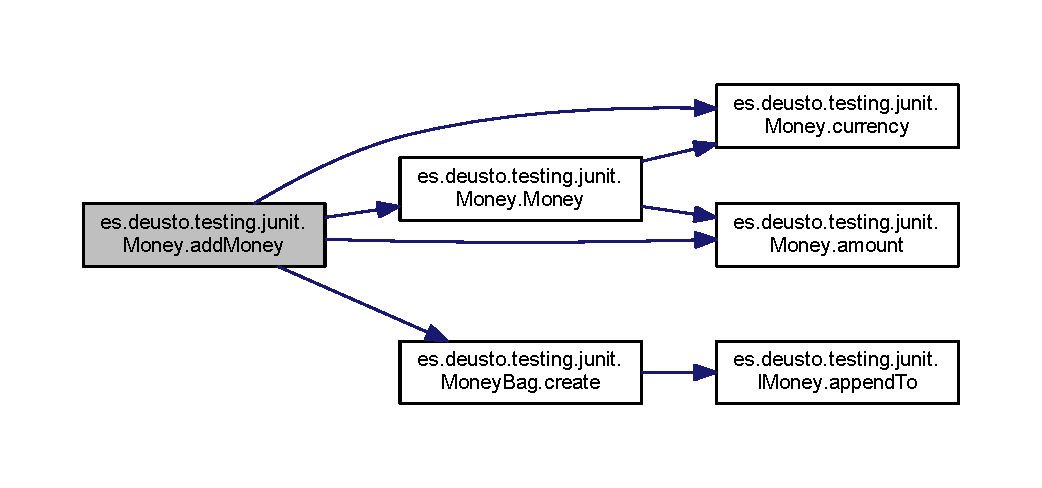
\includegraphics[width=350pt]{classes_1_1deusto_1_1testing_1_1junit_1_1_money_a223a447d5daf23b5e9cc0f551b72e328_cgraph}
\end{center}
\end{figure}
\mbox{\Hypertarget{classes_1_1deusto_1_1testing_1_1junit_1_1_money_ad9a107a6884026a1bb12102d3a8a5b41}\label{classes_1_1deusto_1_1testing_1_1junit_1_1_money_ad9a107a6884026a1bb12102d3a8a5b41}} 
\index{es\+::deusto\+::testing\+::junit\+::\+Money@{es\+::deusto\+::testing\+::junit\+::\+Money}!add\+Money\+Bag@{add\+Money\+Bag}}
\index{add\+Money\+Bag@{add\+Money\+Bag}!es\+::deusto\+::testing\+::junit\+::\+Money@{es\+::deusto\+::testing\+::junit\+::\+Money}}
\subsubsection{\texorpdfstring{add\+Money\+Bag()}{addMoneyBag()}}
{\footnotesize\ttfamily \mbox{\hyperlink{interfacees_1_1deusto_1_1testing_1_1junit_1_1_i_money}{I\+Money}} es.\+deusto.\+testing.\+junit.\+Money.\+add\+Money\+Bag (\begin{DoxyParamCaption}\item[{\mbox{\hyperlink{classes_1_1deusto_1_1testing_1_1junit_1_1_money_bag}{Money\+Bag}}}]{s }\end{DoxyParamCaption})}

Adds a \mbox{\hyperlink{classes_1_1deusto_1_1testing_1_1junit_1_1_money_bag}{Money\+Bag}} to this money. This is a helper method for implementing double dispatch 

Implements \mbox{\hyperlink{interfacees_1_1deusto_1_1testing_1_1junit_1_1_i_money_ac47c8940f0565bd9eda16730170bc9f7}{es.\+deusto.\+testing.\+junit.\+I\+Money}}.



Definition at line 35 of file Money.\+java.

Here is the call graph for this function\+:\nopagebreak
\begin{figure}[H]
\begin{center}
\leavevmode
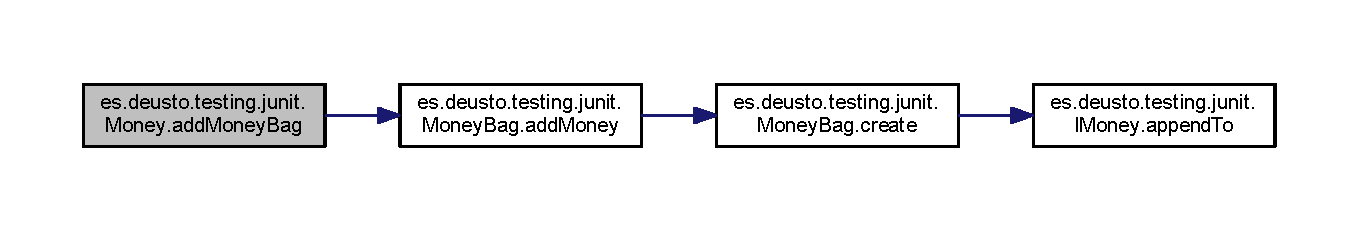
\includegraphics[width=350pt]{classes_1_1deusto_1_1testing_1_1junit_1_1_money_ad9a107a6884026a1bb12102d3a8a5b41_cgraph}
\end{center}
\end{figure}
\mbox{\Hypertarget{classes_1_1deusto_1_1testing_1_1junit_1_1_money_a9bef5d9027f270e8ce0303e4f929bbd5}\label{classes_1_1deusto_1_1testing_1_1junit_1_1_money_a9bef5d9027f270e8ce0303e4f929bbd5}} 
\index{es\+::deusto\+::testing\+::junit\+::\+Money@{es\+::deusto\+::testing\+::junit\+::\+Money}!amount@{amount}}
\index{amount@{amount}!es\+::deusto\+::testing\+::junit\+::\+Money@{es\+::deusto\+::testing\+::junit\+::\+Money}}
\subsubsection{\texorpdfstring{amount()}{amount()}}
{\footnotesize\ttfamily int es.\+deusto.\+testing.\+junit.\+Money.\+amount (\begin{DoxyParamCaption}{ }\end{DoxyParamCaption})}



Definition at line 38 of file Money.\+java.

Here is the caller graph for this function\+:\nopagebreak
\begin{figure}[H]
\begin{center}
\leavevmode
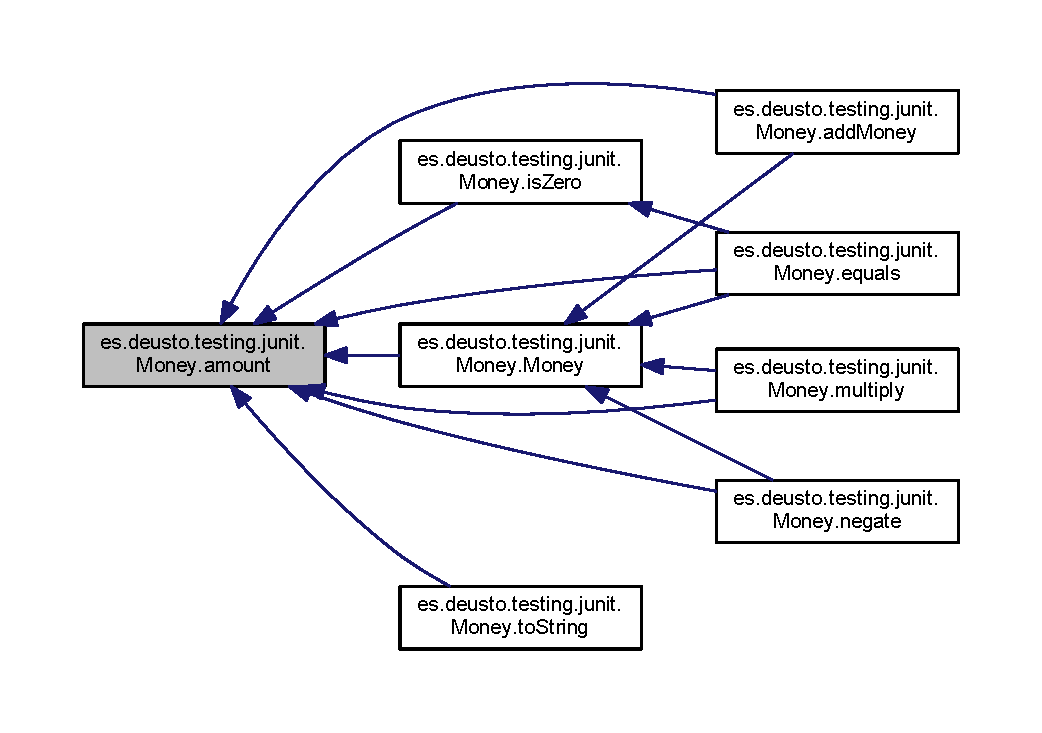
\includegraphics[width=350pt]{classes_1_1deusto_1_1testing_1_1junit_1_1_money_a9bef5d9027f270e8ce0303e4f929bbd5_icgraph}
\end{center}
\end{figure}
\mbox{\Hypertarget{classes_1_1deusto_1_1testing_1_1junit_1_1_money_aa9a6df9f35118060914ae6e8f74d1d51}\label{classes_1_1deusto_1_1testing_1_1junit_1_1_money_aa9a6df9f35118060914ae6e8f74d1d51}} 
\index{es\+::deusto\+::testing\+::junit\+::\+Money@{es\+::deusto\+::testing\+::junit\+::\+Money}!append\+To@{append\+To}}
\index{append\+To@{append\+To}!es\+::deusto\+::testing\+::junit\+::\+Money@{es\+::deusto\+::testing\+::junit\+::\+Money}}
\subsubsection{\texorpdfstring{append\+To()}{appendTo()}}
{\footnotesize\ttfamily void es.\+deusto.\+testing.\+junit.\+Money.\+append\+To (\begin{DoxyParamCaption}\item[{\mbox{\hyperlink{classes_1_1deusto_1_1testing_1_1junit_1_1_money_bag}{Money\+Bag}}}]{m }\end{DoxyParamCaption})}

This makes no sense May 12, 2014 

Implements \mbox{\hyperlink{interfacees_1_1deusto_1_1testing_1_1junit_1_1_i_money_ae45bc758e69a0017f083f11d050c53cb}{es.\+deusto.\+testing.\+junit.\+I\+Money}}.



Definition at line 80 of file Money.\+java.

\mbox{\Hypertarget{classes_1_1deusto_1_1testing_1_1junit_1_1_money_aefa4aaf62bb653eae25851d98ae02dcb}\label{classes_1_1deusto_1_1testing_1_1junit_1_1_money_aefa4aaf62bb653eae25851d98ae02dcb}} 
\index{es\+::deusto\+::testing\+::junit\+::\+Money@{es\+::deusto\+::testing\+::junit\+::\+Money}!currency@{currency}}
\index{currency@{currency}!es\+::deusto\+::testing\+::junit\+::\+Money@{es\+::deusto\+::testing\+::junit\+::\+Money}}
\subsubsection{\texorpdfstring{currency()}{currency()}}
{\footnotesize\ttfamily String es.\+deusto.\+testing.\+junit.\+Money.\+currency (\begin{DoxyParamCaption}{ }\end{DoxyParamCaption})}



Definition at line 41 of file Money.\+java.

Here is the caller graph for this function\+:\nopagebreak
\begin{figure}[H]
\begin{center}
\leavevmode
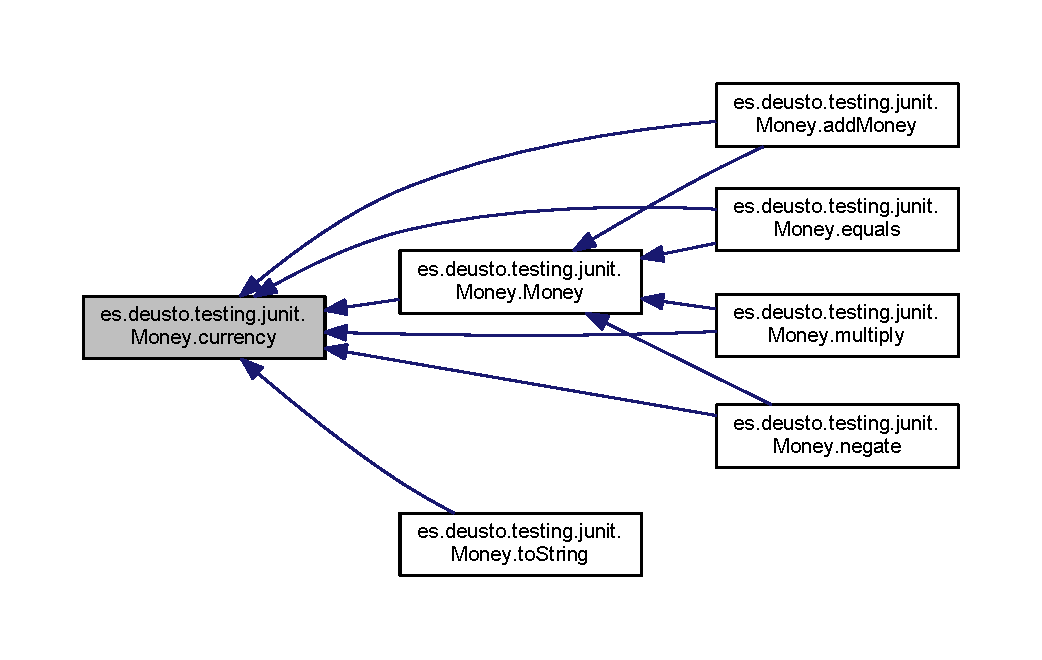
\includegraphics[width=350pt]{classes_1_1deusto_1_1testing_1_1junit_1_1_money_aefa4aaf62bb653eae25851d98ae02dcb_icgraph}
\end{center}
\end{figure}
\mbox{\Hypertarget{classes_1_1deusto_1_1testing_1_1junit_1_1_money_a2356df38b8e9ecdd969bab11d6dd301b}\label{classes_1_1deusto_1_1testing_1_1junit_1_1_money_a2356df38b8e9ecdd969bab11d6dd301b}} 
\index{es\+::deusto\+::testing\+::junit\+::\+Money@{es\+::deusto\+::testing\+::junit\+::\+Money}!equals@{equals}}
\index{equals@{equals}!es\+::deusto\+::testing\+::junit\+::\+Money@{es\+::deusto\+::testing\+::junit\+::\+Money}}
\subsubsection{\texorpdfstring{equals()}{equals()}}
{\footnotesize\ttfamily boolean es.\+deusto.\+testing.\+junit.\+Money.\+equals (\begin{DoxyParamCaption}\item[{Object}]{an\+Object }\end{DoxyParamCaption})}



Definition at line 45 of file Money.\+java.

Here is the call graph for this function\+:\nopagebreak
\begin{figure}[H]
\begin{center}
\leavevmode
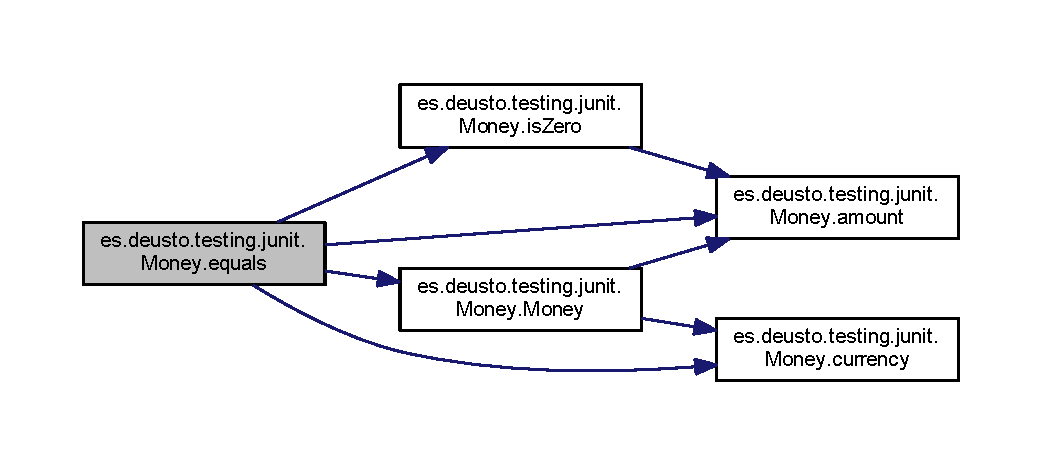
\includegraphics[width=350pt]{classes_1_1deusto_1_1testing_1_1junit_1_1_money_a2356df38b8e9ecdd969bab11d6dd301b_cgraph}
\end{center}
\end{figure}
\mbox{\Hypertarget{classes_1_1deusto_1_1testing_1_1junit_1_1_money_af6cfb5b27bf97170d990dea12de04f37}\label{classes_1_1deusto_1_1testing_1_1junit_1_1_money_af6cfb5b27bf97170d990dea12de04f37}} 
\index{es\+::deusto\+::testing\+::junit\+::\+Money@{es\+::deusto\+::testing\+::junit\+::\+Money}!hash\+Code@{hash\+Code}}
\index{hash\+Code@{hash\+Code}!es\+::deusto\+::testing\+::junit\+::\+Money@{es\+::deusto\+::testing\+::junit\+::\+Money}}
\subsubsection{\texorpdfstring{hash\+Code()}{hashCode()}}
{\footnotesize\ttfamily int es.\+deusto.\+testing.\+junit.\+Money.\+hash\+Code (\begin{DoxyParamCaption}{ }\end{DoxyParamCaption})}



Definition at line 57 of file Money.\+java.

\mbox{\Hypertarget{classes_1_1deusto_1_1testing_1_1junit_1_1_money_a797658a03260b535e9a36ebbcc3b19c9}\label{classes_1_1deusto_1_1testing_1_1junit_1_1_money_a797658a03260b535e9a36ebbcc3b19c9}} 
\index{es\+::deusto\+::testing\+::junit\+::\+Money@{es\+::deusto\+::testing\+::junit\+::\+Money}!is\+Zero@{is\+Zero}}
\index{is\+Zero@{is\+Zero}!es\+::deusto\+::testing\+::junit\+::\+Money@{es\+::deusto\+::testing\+::junit\+::\+Money}}
\subsubsection{\texorpdfstring{is\+Zero()}{isZero()}}
{\footnotesize\ttfamily boolean es.\+deusto.\+testing.\+junit.\+Money.\+is\+Zero (\begin{DoxyParamCaption}{ }\end{DoxyParamCaption})}

Tests whether this money is zero 

Implements \mbox{\hyperlink{interfacees_1_1deusto_1_1testing_1_1junit_1_1_i_money_a166c39b6f931e49769580a04f8c73500}{es.\+deusto.\+testing.\+junit.\+I\+Money}}.



Definition at line 62 of file Money.\+java.

Here is the call graph for this function\+:\nopagebreak
\begin{figure}[H]
\begin{center}
\leavevmode
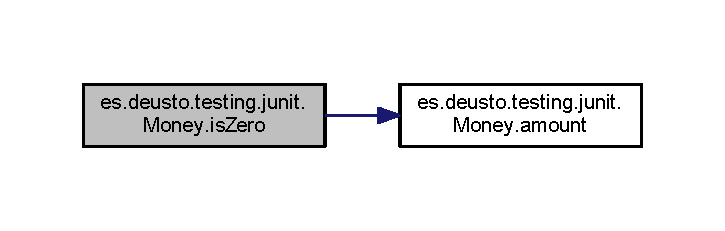
\includegraphics[width=348pt]{classes_1_1deusto_1_1testing_1_1junit_1_1_money_a797658a03260b535e9a36ebbcc3b19c9_cgraph}
\end{center}
\end{figure}
Here is the caller graph for this function\+:\nopagebreak
\begin{figure}[H]
\begin{center}
\leavevmode
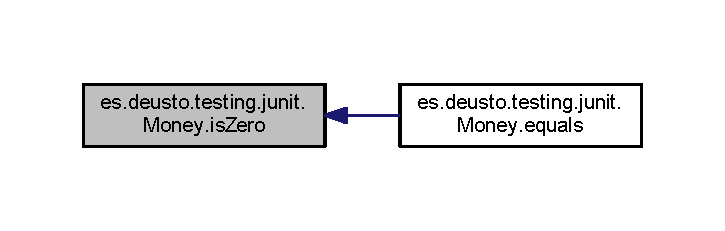
\includegraphics[width=348pt]{classes_1_1deusto_1_1testing_1_1junit_1_1_money_a797658a03260b535e9a36ebbcc3b19c9_icgraph}
\end{center}
\end{figure}
\mbox{\Hypertarget{classes_1_1deusto_1_1testing_1_1junit_1_1_money_a02c7d4e9013710f70d1d46e9c9ebae88}\label{classes_1_1deusto_1_1testing_1_1junit_1_1_money_a02c7d4e9013710f70d1d46e9c9ebae88}} 
\index{es\+::deusto\+::testing\+::junit\+::\+Money@{es\+::deusto\+::testing\+::junit\+::\+Money}!multiply@{multiply}}
\index{multiply@{multiply}!es\+::deusto\+::testing\+::junit\+::\+Money@{es\+::deusto\+::testing\+::junit\+::\+Money}}
\subsubsection{\texorpdfstring{multiply()}{multiply()}}
{\footnotesize\ttfamily \mbox{\hyperlink{interfacees_1_1deusto_1_1testing_1_1junit_1_1_i_money}{I\+Money}} es.\+deusto.\+testing.\+junit.\+Money.\+multiply (\begin{DoxyParamCaption}\item[{int}]{factor }\end{DoxyParamCaption})}

Multiplies a money by the given factor. 

Implements \mbox{\hyperlink{interfacees_1_1deusto_1_1testing_1_1junit_1_1_i_money_a09154f9713133d4734f72d6a20081209}{es.\+deusto.\+testing.\+junit.\+I\+Money}}.



Definition at line 65 of file Money.\+java.

Here is the call graph for this function\+:\nopagebreak
\begin{figure}[H]
\begin{center}
\leavevmode
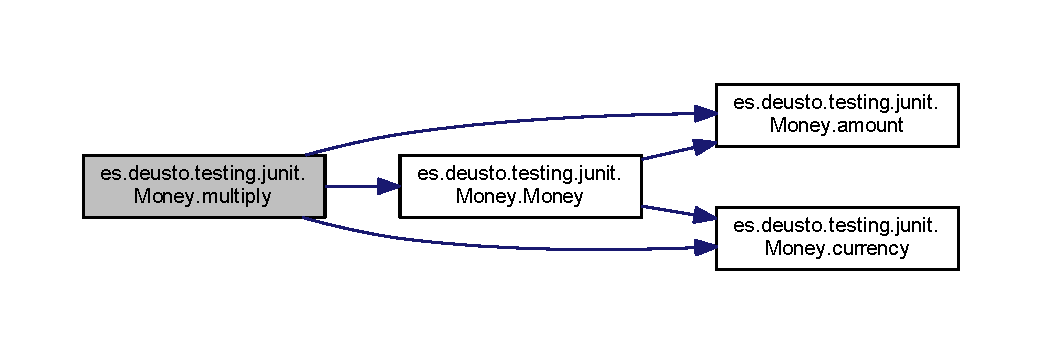
\includegraphics[width=350pt]{classes_1_1deusto_1_1testing_1_1junit_1_1_money_a02c7d4e9013710f70d1d46e9c9ebae88_cgraph}
\end{center}
\end{figure}
\mbox{\Hypertarget{classes_1_1deusto_1_1testing_1_1junit_1_1_money_ae5f0bc3ea87f1fd55d6478653b8f2e36}\label{classes_1_1deusto_1_1testing_1_1junit_1_1_money_ae5f0bc3ea87f1fd55d6478653b8f2e36}} 
\index{es\+::deusto\+::testing\+::junit\+::\+Money@{es\+::deusto\+::testing\+::junit\+::\+Money}!negate@{negate}}
\index{negate@{negate}!es\+::deusto\+::testing\+::junit\+::\+Money@{es\+::deusto\+::testing\+::junit\+::\+Money}}
\subsubsection{\texorpdfstring{negate()}{negate()}}
{\footnotesize\ttfamily \mbox{\hyperlink{interfacees_1_1deusto_1_1testing_1_1junit_1_1_i_money}{I\+Money}} es.\+deusto.\+testing.\+junit.\+Money.\+negate (\begin{DoxyParamCaption}{ }\end{DoxyParamCaption})}

Negates this money. 

Implements \mbox{\hyperlink{interfacees_1_1deusto_1_1testing_1_1junit_1_1_i_money_a741967d7aa89055b6873619303b11385}{es.\+deusto.\+testing.\+junit.\+I\+Money}}.



Definition at line 68 of file Money.\+java.

Here is the call graph for this function\+:\nopagebreak
\begin{figure}[H]
\begin{center}
\leavevmode
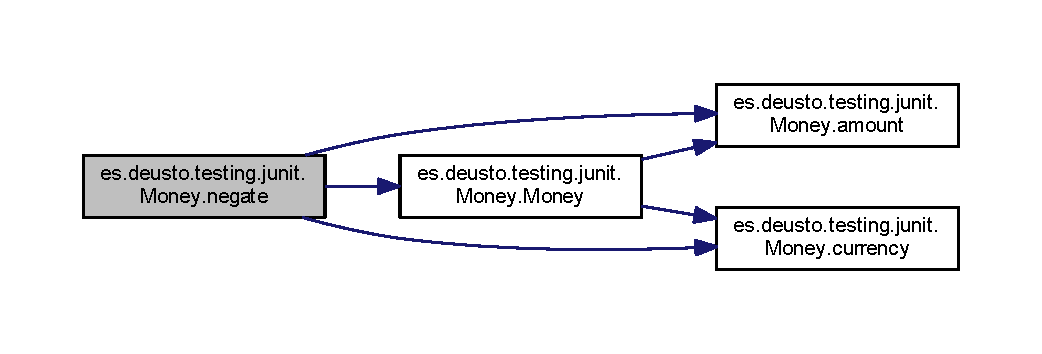
\includegraphics[width=350pt]{classes_1_1deusto_1_1testing_1_1junit_1_1_money_ae5f0bc3ea87f1fd55d6478653b8f2e36_cgraph}
\end{center}
\end{figure}
\mbox{\Hypertarget{classes_1_1deusto_1_1testing_1_1junit_1_1_money_aada973cd1a31410ed2b7e5d2ae6bc2e9}\label{classes_1_1deusto_1_1testing_1_1junit_1_1_money_aada973cd1a31410ed2b7e5d2ae6bc2e9}} 
\index{es\+::deusto\+::testing\+::junit\+::\+Money@{es\+::deusto\+::testing\+::junit\+::\+Money}!subtract@{subtract}}
\index{subtract@{subtract}!es\+::deusto\+::testing\+::junit\+::\+Money@{es\+::deusto\+::testing\+::junit\+::\+Money}}
\subsubsection{\texorpdfstring{subtract()}{subtract()}}
{\footnotesize\ttfamily \mbox{\hyperlink{interfacees_1_1deusto_1_1testing_1_1junit_1_1_i_money}{I\+Money}} es.\+deusto.\+testing.\+junit.\+Money.\+subtract (\begin{DoxyParamCaption}\item[{\mbox{\hyperlink{interfacees_1_1deusto_1_1testing_1_1junit_1_1_i_money}{I\+Money}}}]{m }\end{DoxyParamCaption})}

Subtracts a money from this money. 

Implements \mbox{\hyperlink{interfacees_1_1deusto_1_1testing_1_1junit_1_1_i_money_a1fb4981aa759e3fe0679654bec7a8b61}{es.\+deusto.\+testing.\+junit.\+I\+Money}}.



Definition at line 71 of file Money.\+java.

Here is the call graph for this function\+:\nopagebreak
\begin{figure}[H]
\begin{center}
\leavevmode
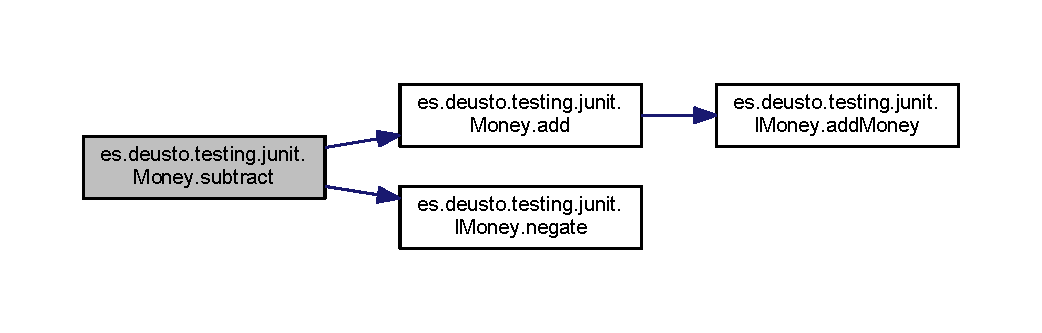
\includegraphics[width=350pt]{classes_1_1deusto_1_1testing_1_1junit_1_1_money_aada973cd1a31410ed2b7e5d2ae6bc2e9_cgraph}
\end{center}
\end{figure}
\mbox{\Hypertarget{classes_1_1deusto_1_1testing_1_1junit_1_1_money_af9e655069123757bea0efecc4efcd638}\label{classes_1_1deusto_1_1testing_1_1junit_1_1_money_af9e655069123757bea0efecc4efcd638}} 
\index{es\+::deusto\+::testing\+::junit\+::\+Money@{es\+::deusto\+::testing\+::junit\+::\+Money}!to\+String@{to\+String}}
\index{to\+String@{to\+String}!es\+::deusto\+::testing\+::junit\+::\+Money@{es\+::deusto\+::testing\+::junit\+::\+Money}}
\subsubsection{\texorpdfstring{to\+String()}{toString()}}
{\footnotesize\ttfamily String es.\+deusto.\+testing.\+junit.\+Money.\+to\+String (\begin{DoxyParamCaption}{ }\end{DoxyParamCaption})}



Definition at line 75 of file Money.\+java.

Here is the call graph for this function\+:\nopagebreak
\begin{figure}[H]
\begin{center}
\leavevmode
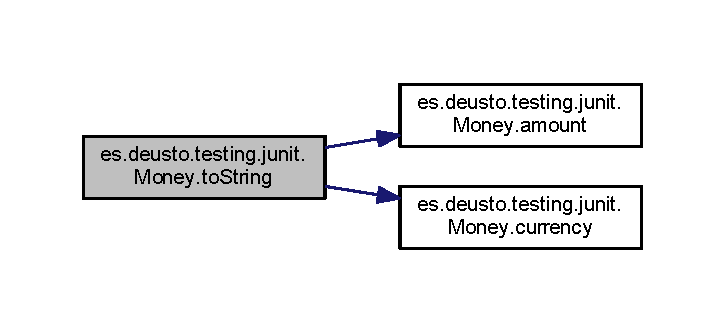
\includegraphics[width=348pt]{classes_1_1deusto_1_1testing_1_1junit_1_1_money_af9e655069123757bea0efecc4efcd638_cgraph}
\end{center}
\end{figure}


The documentation for this class was generated from the following file\+:\begin{DoxyCompactItemize}
\item 
src/main/java/es/deusto/testing/junit/\mbox{\hyperlink{_money_8java}{Money.\+java}}\end{DoxyCompactItemize}

\hypertarget{classes_1_1deusto_1_1testing_1_1junit_1_1_money_bag}{}\section{es.\+deusto.\+testing.\+junit.\+Money\+Bag Class Reference}
\label{classes_1_1deusto_1_1testing_1_1junit_1_1_money_bag}\index{es.\+deusto.\+testing.\+junit.\+Money\+Bag@{es.\+deusto.\+testing.\+junit.\+Money\+Bag}}


Inheritance diagram for es.\+deusto.\+testing.\+junit.\+Money\+Bag\+:\nopagebreak
\begin{figure}[H]
\begin{center}
\leavevmode
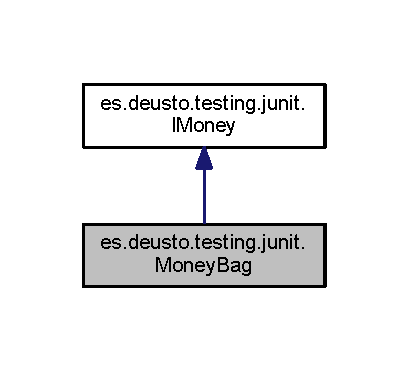
\includegraphics[width=196pt]{classes_1_1deusto_1_1testing_1_1junit_1_1_money_bag__inherit__graph}
\end{center}
\end{figure}


Collaboration diagram for es.\+deusto.\+testing.\+junit.\+Money\+Bag\+:\nopagebreak
\begin{figure}[H]
\begin{center}
\leavevmode
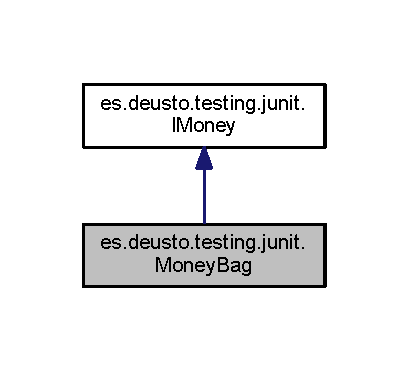
\includegraphics[width=196pt]{classes_1_1deusto_1_1testing_1_1junit_1_1_money_bag__coll__graph}
\end{center}
\end{figure}
\subsection*{Public Member Functions}
\begin{DoxyCompactItemize}
\item 
\mbox{\hyperlink{interfacees_1_1deusto_1_1testing_1_1junit_1_1_i_money}{I\+Money}} \mbox{\hyperlink{classes_1_1deusto_1_1testing_1_1junit_1_1_money_bag_ab3be83ff12fa6d19b67b669194120d00}{add}} (\mbox{\hyperlink{interfacees_1_1deusto_1_1testing_1_1junit_1_1_i_money}{I\+Money}} m)
\item 
\mbox{\hyperlink{interfacees_1_1deusto_1_1testing_1_1junit_1_1_i_money}{I\+Money}} \mbox{\hyperlink{classes_1_1deusto_1_1testing_1_1junit_1_1_money_bag_a06ecedbf53ba09d34276fe177e3169bc}{add\+Money}} (\mbox{\hyperlink{classes_1_1deusto_1_1testing_1_1junit_1_1_money}{Money}} m)
\item 
\mbox{\hyperlink{interfacees_1_1deusto_1_1testing_1_1junit_1_1_i_money}{I\+Money}} \mbox{\hyperlink{classes_1_1deusto_1_1testing_1_1junit_1_1_money_bag_ab329e6a2811b83a2b1670b79be92249d}{add\+Money\+Bag}} (\mbox{\hyperlink{classes_1_1deusto_1_1testing_1_1junit_1_1_money_bag}{Money\+Bag}} s)
\item 
boolean \mbox{\hyperlink{classes_1_1deusto_1_1testing_1_1junit_1_1_money_bag_a80926d10c9619bd2ad84eabe52ca03bb}{equals}} (Object an\+Object)
\item 
int \mbox{\hyperlink{classes_1_1deusto_1_1testing_1_1junit_1_1_money_bag_ae2c0d290a37a617f0a07134bf95162eb}{hash\+Code}} ()
\item 
boolean \mbox{\hyperlink{classes_1_1deusto_1_1testing_1_1junit_1_1_money_bag_abebc5bc39c3343cb3c4e5fb291fd5893}{is\+Zero}} ()
\item 
\mbox{\hyperlink{interfacees_1_1deusto_1_1testing_1_1junit_1_1_i_money}{I\+Money}} \mbox{\hyperlink{classes_1_1deusto_1_1testing_1_1junit_1_1_money_bag_aa20ce4cc70c2ba0bc9a5ccb96635d506}{multiply}} (int factor)
\item 
\mbox{\hyperlink{interfacees_1_1deusto_1_1testing_1_1junit_1_1_i_money}{I\+Money}} \mbox{\hyperlink{classes_1_1deusto_1_1testing_1_1junit_1_1_money_bag_abf06bf97e548f95038756608fe0c8351}{negate}} ()
\item 
\mbox{\hyperlink{interfacees_1_1deusto_1_1testing_1_1junit_1_1_i_money}{I\+Money}} \mbox{\hyperlink{classes_1_1deusto_1_1testing_1_1junit_1_1_money_bag_a7f1803fe267edca895cdf752b5f46560}{subtract}} (\mbox{\hyperlink{interfacees_1_1deusto_1_1testing_1_1junit_1_1_i_money}{I\+Money}} m)
\item 
String \mbox{\hyperlink{classes_1_1deusto_1_1testing_1_1junit_1_1_money_bag_a85b49bdc3ff191abdaa1ad1a065ec5f1}{to\+String}} ()
\item 
void \mbox{\hyperlink{classes_1_1deusto_1_1testing_1_1junit_1_1_money_bag_ac8a5877b35b12939ce14543872ed18af}{append\+To}} (\mbox{\hyperlink{classes_1_1deusto_1_1testing_1_1junit_1_1_money_bag}{Money\+Bag}} m)
\begin{DoxyCompactList}\small\item\em Brief test for \mbox{\hyperlink{classes_1_1deusto_1_1testing_1_1junit_1_1_money_bag_ac8a5877b35b12939ce14543872ed18af}{append\+To()}} added May 12, 2014. \end{DoxyCompactList}\end{DoxyCompactItemize}
\subsection*{Static Public Member Functions}
\begin{DoxyCompactItemize}
\item 
static \mbox{\hyperlink{interfacees_1_1deusto_1_1testing_1_1junit_1_1_i_money}{I\+Money}} \mbox{\hyperlink{classes_1_1deusto_1_1testing_1_1junit_1_1_money_bag_a8d2d54a342d2de2b75530600123efc9a}{create}} (\mbox{\hyperlink{interfacees_1_1deusto_1_1testing_1_1junit_1_1_i_money}{I\+Money}} m1, \mbox{\hyperlink{interfacees_1_1deusto_1_1testing_1_1junit_1_1_i_money}{I\+Money}} m2)
\end{DoxyCompactItemize}


\subsection{Detailed Description}
A \mbox{\hyperlink{classes_1_1deusto_1_1testing_1_1junit_1_1_money_bag}{Money\+Bag}} defers exchange rate conversions. For example adding 12 Swiss Francs to 14 US Dollars is represented as a bag containing the two \mbox{\hyperlink{classes_1_1deusto_1_1testing_1_1junit_1_1_money}{Money}} objects associated to 12 C\+HF and 14 U\+SD. Adding another 10 Swiss francs gives a \mbox{\hyperlink{classes_1_1deusto_1_1testing_1_1junit_1_1_money_bag}{Money\+Bag}} with 22 C\+HF and 14 U\+SD. Due to the deferred exchange rate conversion we can later value a \mbox{\hyperlink{classes_1_1deusto_1_1testing_1_1junit_1_1_money_bag}{Money\+Bag}} with different exchange rates.

A \mbox{\hyperlink{classes_1_1deusto_1_1testing_1_1junit_1_1_money_bag}{Money\+Bag}} is represented as a list of \mbox{\hyperlink{classes_1_1deusto_1_1testing_1_1junit_1_1_money}{Money}} objects and provides different constructors to create a \mbox{\hyperlink{classes_1_1deusto_1_1testing_1_1junit_1_1_money_bag}{Money\+Bag}}. 

Definition at line 23 of file Money\+Bag.\+java.



\subsection{Member Function Documentation}
\mbox{\Hypertarget{classes_1_1deusto_1_1testing_1_1junit_1_1_money_bag_ab3be83ff12fa6d19b67b669194120d00}\label{classes_1_1deusto_1_1testing_1_1junit_1_1_money_bag_ab3be83ff12fa6d19b67b669194120d00}} 
\index{es\+::deusto\+::testing\+::junit\+::\+Money\+Bag@{es\+::deusto\+::testing\+::junit\+::\+Money\+Bag}!add@{add}}
\index{add@{add}!es\+::deusto\+::testing\+::junit\+::\+Money\+Bag@{es\+::deusto\+::testing\+::junit\+::\+Money\+Bag}}
\subsubsection{\texorpdfstring{add()}{add()}}
{\footnotesize\ttfamily \mbox{\hyperlink{interfacees_1_1deusto_1_1testing_1_1junit_1_1_i_money}{I\+Money}} es.\+deusto.\+testing.\+junit.\+Money\+Bag.\+add (\begin{DoxyParamCaption}\item[{\mbox{\hyperlink{interfacees_1_1deusto_1_1testing_1_1junit_1_1_i_money}{I\+Money}}}]{m }\end{DoxyParamCaption})}

Adds a money to this money. 

Implements \mbox{\hyperlink{interfacees_1_1deusto_1_1testing_1_1junit_1_1_i_money_a7f3ac1ced239e64294706155c569b8de}{es.\+deusto.\+testing.\+junit.\+I\+Money}}.



Definition at line 32 of file Money\+Bag.\+java.

Here is the call graph for this function\+:\nopagebreak
\begin{figure}[H]
\begin{center}
\leavevmode
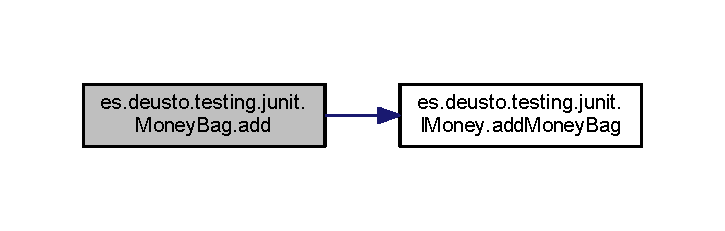
\includegraphics[width=348pt]{classes_1_1deusto_1_1testing_1_1junit_1_1_money_bag_ab3be83ff12fa6d19b67b669194120d00_cgraph}
\end{center}
\end{figure}
Here is the caller graph for this function\+:\nopagebreak
\begin{figure}[H]
\begin{center}
\leavevmode
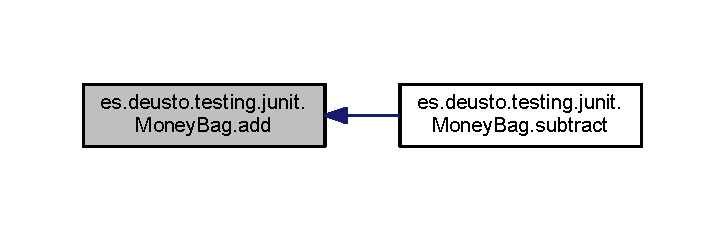
\includegraphics[width=348pt]{classes_1_1deusto_1_1testing_1_1junit_1_1_money_bag_ab3be83ff12fa6d19b67b669194120d00_icgraph}
\end{center}
\end{figure}
\mbox{\Hypertarget{classes_1_1deusto_1_1testing_1_1junit_1_1_money_bag_a06ecedbf53ba09d34276fe177e3169bc}\label{classes_1_1deusto_1_1testing_1_1junit_1_1_money_bag_a06ecedbf53ba09d34276fe177e3169bc}} 
\index{es\+::deusto\+::testing\+::junit\+::\+Money\+Bag@{es\+::deusto\+::testing\+::junit\+::\+Money\+Bag}!add\+Money@{add\+Money}}
\index{add\+Money@{add\+Money}!es\+::deusto\+::testing\+::junit\+::\+Money\+Bag@{es\+::deusto\+::testing\+::junit\+::\+Money\+Bag}}
\subsubsection{\texorpdfstring{add\+Money()}{addMoney()}}
{\footnotesize\ttfamily \mbox{\hyperlink{interfacees_1_1deusto_1_1testing_1_1junit_1_1_i_money}{I\+Money}} es.\+deusto.\+testing.\+junit.\+Money\+Bag.\+add\+Money (\begin{DoxyParamCaption}\item[{\mbox{\hyperlink{classes_1_1deusto_1_1testing_1_1junit_1_1_money}{Money}}}]{m }\end{DoxyParamCaption})}

Adds a simple \mbox{\hyperlink{classes_1_1deusto_1_1testing_1_1junit_1_1_money}{Money}} to this money. This is a helper method for implementing double dispatch 

Implements \mbox{\hyperlink{interfacees_1_1deusto_1_1testing_1_1junit_1_1_i_money_aab8d4be667a542a8aa1380eb2b6e4257}{es.\+deusto.\+testing.\+junit.\+I\+Money}}.



Definition at line 35 of file Money\+Bag.\+java.

Here is the call graph for this function\+:\nopagebreak
\begin{figure}[H]
\begin{center}
\leavevmode
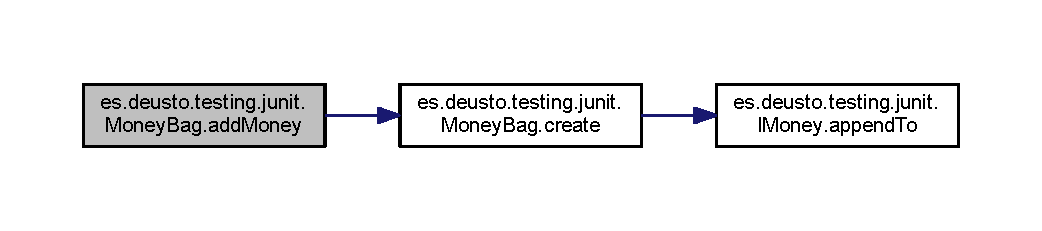
\includegraphics[width=350pt]{classes_1_1deusto_1_1testing_1_1junit_1_1_money_bag_a06ecedbf53ba09d34276fe177e3169bc_cgraph}
\end{center}
\end{figure}
Here is the caller graph for this function\+:\nopagebreak
\begin{figure}[H]
\begin{center}
\leavevmode
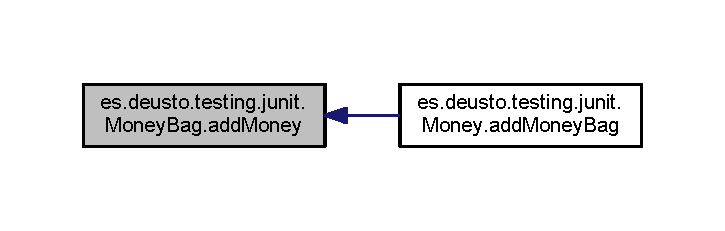
\includegraphics[width=348pt]{classes_1_1deusto_1_1testing_1_1junit_1_1_money_bag_a06ecedbf53ba09d34276fe177e3169bc_icgraph}
\end{center}
\end{figure}
\mbox{\Hypertarget{classes_1_1deusto_1_1testing_1_1junit_1_1_money_bag_ab329e6a2811b83a2b1670b79be92249d}\label{classes_1_1deusto_1_1testing_1_1junit_1_1_money_bag_ab329e6a2811b83a2b1670b79be92249d}} 
\index{es\+::deusto\+::testing\+::junit\+::\+Money\+Bag@{es\+::deusto\+::testing\+::junit\+::\+Money\+Bag}!add\+Money\+Bag@{add\+Money\+Bag}}
\index{add\+Money\+Bag@{add\+Money\+Bag}!es\+::deusto\+::testing\+::junit\+::\+Money\+Bag@{es\+::deusto\+::testing\+::junit\+::\+Money\+Bag}}
\subsubsection{\texorpdfstring{add\+Money\+Bag()}{addMoneyBag()}}
{\footnotesize\ttfamily \mbox{\hyperlink{interfacees_1_1deusto_1_1testing_1_1junit_1_1_i_money}{I\+Money}} es.\+deusto.\+testing.\+junit.\+Money\+Bag.\+add\+Money\+Bag (\begin{DoxyParamCaption}\item[{\mbox{\hyperlink{classes_1_1deusto_1_1testing_1_1junit_1_1_money_bag}{Money\+Bag}}}]{s }\end{DoxyParamCaption})}

Adds a \mbox{\hyperlink{classes_1_1deusto_1_1testing_1_1junit_1_1_money_bag}{Money\+Bag}} to this money. This is a helper method for implementing double dispatch 

Implements \mbox{\hyperlink{interfacees_1_1deusto_1_1testing_1_1junit_1_1_i_money_ac47c8940f0565bd9eda16730170bc9f7}{es.\+deusto.\+testing.\+junit.\+I\+Money}}.



Definition at line 38 of file Money\+Bag.\+java.

Here is the call graph for this function\+:\nopagebreak
\begin{figure}[H]
\begin{center}
\leavevmode
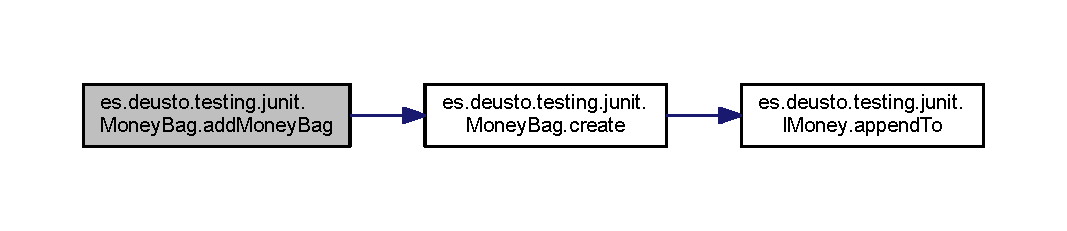
\includegraphics[width=350pt]{classes_1_1deusto_1_1testing_1_1junit_1_1_money_bag_ab329e6a2811b83a2b1670b79be92249d_cgraph}
\end{center}
\end{figure}
\mbox{\Hypertarget{classes_1_1deusto_1_1testing_1_1junit_1_1_money_bag_ac8a5877b35b12939ce14543872ed18af}\label{classes_1_1deusto_1_1testing_1_1junit_1_1_money_bag_ac8a5877b35b12939ce14543872ed18af}} 
\index{es\+::deusto\+::testing\+::junit\+::\+Money\+Bag@{es\+::deusto\+::testing\+::junit\+::\+Money\+Bag}!append\+To@{append\+To}}
\index{append\+To@{append\+To}!es\+::deusto\+::testing\+::junit\+::\+Money\+Bag@{es\+::deusto\+::testing\+::junit\+::\+Money\+Bag}}
\subsubsection{\texorpdfstring{append\+To()}{appendTo()}}
{\footnotesize\ttfamily void es.\+deusto.\+testing.\+junit.\+Money\+Bag.\+append\+To (\begin{DoxyParamCaption}\item[{\mbox{\hyperlink{classes_1_1deusto_1_1testing_1_1junit_1_1_money_bag}{Money\+Bag}}}]{m }\end{DoxyParamCaption})}



Brief test for \mbox{\hyperlink{classes_1_1deusto_1_1testing_1_1junit_1_1_money_bag_ac8a5877b35b12939ce14543872ed18af}{append\+To()}} added May 12, 2014. 

Append this to a \mbox{\hyperlink{classes_1_1deusto_1_1testing_1_1junit_1_1_money_bag}{Money\+Bag}} m. \mbox{\hyperlink{classes_1_1deusto_1_1testing_1_1junit_1_1_money_bag_ac8a5877b35b12939ce14543872ed18af}{append\+To()}} needs to be public because it is used polymorphically, but it should not be used by clients because it modifies the argument m. 

Implements \mbox{\hyperlink{interfacees_1_1deusto_1_1testing_1_1junit_1_1_i_money_ae45bc758e69a0017f083f11d050c53cb}{es.\+deusto.\+testing.\+junit.\+I\+Money}}.



Definition at line 127 of file Money\+Bag.\+java.

\mbox{\Hypertarget{classes_1_1deusto_1_1testing_1_1junit_1_1_money_bag_a8d2d54a342d2de2b75530600123efc9a}\label{classes_1_1deusto_1_1testing_1_1junit_1_1_money_bag_a8d2d54a342d2de2b75530600123efc9a}} 
\index{es\+::deusto\+::testing\+::junit\+::\+Money\+Bag@{es\+::deusto\+::testing\+::junit\+::\+Money\+Bag}!create@{create}}
\index{create@{create}!es\+::deusto\+::testing\+::junit\+::\+Money\+Bag@{es\+::deusto\+::testing\+::junit\+::\+Money\+Bag}}
\subsubsection{\texorpdfstring{create()}{create()}}
{\footnotesize\ttfamily static \mbox{\hyperlink{interfacees_1_1deusto_1_1testing_1_1junit_1_1_i_money}{I\+Money}} es.\+deusto.\+testing.\+junit.\+Money\+Bag.\+create (\begin{DoxyParamCaption}\item[{\mbox{\hyperlink{interfacees_1_1deusto_1_1testing_1_1junit_1_1_i_money}{I\+Money}}}]{m1,  }\item[{\mbox{\hyperlink{interfacees_1_1deusto_1_1testing_1_1junit_1_1_i_money}{I\+Money}}}]{m2 }\end{DoxyParamCaption})\hspace{0.3cm}{\ttfamily [static]}}



Definition at line 26 of file Money\+Bag.\+java.

Here is the call graph for this function\+:\nopagebreak
\begin{figure}[H]
\begin{center}
\leavevmode
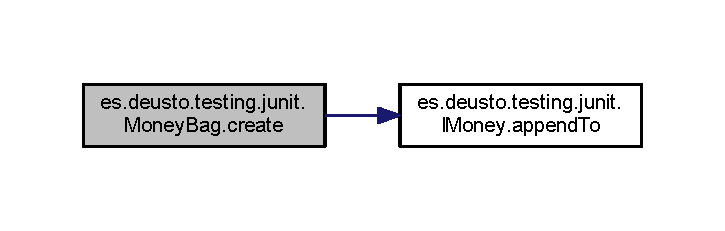
\includegraphics[width=348pt]{classes_1_1deusto_1_1testing_1_1junit_1_1_money_bag_a8d2d54a342d2de2b75530600123efc9a_cgraph}
\end{center}
\end{figure}
Here is the caller graph for this function\+:\nopagebreak
\begin{figure}[H]
\begin{center}
\leavevmode
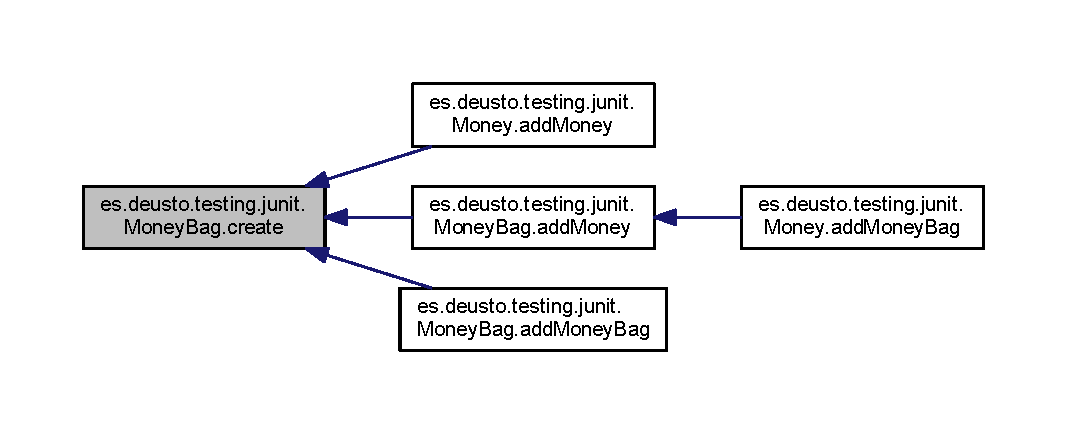
\includegraphics[width=350pt]{classes_1_1deusto_1_1testing_1_1junit_1_1_money_bag_a8d2d54a342d2de2b75530600123efc9a_icgraph}
\end{center}
\end{figure}
\mbox{\Hypertarget{classes_1_1deusto_1_1testing_1_1junit_1_1_money_bag_a80926d10c9619bd2ad84eabe52ca03bb}\label{classes_1_1deusto_1_1testing_1_1junit_1_1_money_bag_a80926d10c9619bd2ad84eabe52ca03bb}} 
\index{es\+::deusto\+::testing\+::junit\+::\+Money\+Bag@{es\+::deusto\+::testing\+::junit\+::\+Money\+Bag}!equals@{equals}}
\index{equals@{equals}!es\+::deusto\+::testing\+::junit\+::\+Money\+Bag@{es\+::deusto\+::testing\+::junit\+::\+Money\+Bag}}
\subsubsection{\texorpdfstring{equals()}{equals()}}
{\footnotesize\ttfamily boolean es.\+deusto.\+testing.\+junit.\+Money\+Bag.\+equals (\begin{DoxyParamCaption}\item[{Object}]{an\+Object }\end{DoxyParamCaption})}



Definition at line 59 of file Money\+Bag.\+java.

Here is the call graph for this function\+:\nopagebreak
\begin{figure}[H]
\begin{center}
\leavevmode
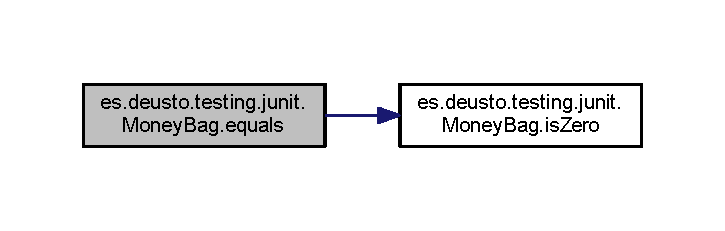
\includegraphics[width=348pt]{classes_1_1deusto_1_1testing_1_1junit_1_1_money_bag_a80926d10c9619bd2ad84eabe52ca03bb_cgraph}
\end{center}
\end{figure}
\mbox{\Hypertarget{classes_1_1deusto_1_1testing_1_1junit_1_1_money_bag_ae2c0d290a37a617f0a07134bf95162eb}\label{classes_1_1deusto_1_1testing_1_1junit_1_1_money_bag_ae2c0d290a37a617f0a07134bf95162eb}} 
\index{es\+::deusto\+::testing\+::junit\+::\+Money\+Bag@{es\+::deusto\+::testing\+::junit\+::\+Money\+Bag}!hash\+Code@{hash\+Code}}
\index{hash\+Code@{hash\+Code}!es\+::deusto\+::testing\+::junit\+::\+Money\+Bag@{es\+::deusto\+::testing\+::junit\+::\+Money\+Bag}}
\subsubsection{\texorpdfstring{hash\+Code()}{hashCode()}}
{\footnotesize\ttfamily int es.\+deusto.\+testing.\+junit.\+Money\+Bag.\+hash\+Code (\begin{DoxyParamCaption}{ }\end{DoxyParamCaption})}



Definition at line 88 of file Money\+Bag.\+java.

\mbox{\Hypertarget{classes_1_1deusto_1_1testing_1_1junit_1_1_money_bag_abebc5bc39c3343cb3c4e5fb291fd5893}\label{classes_1_1deusto_1_1testing_1_1junit_1_1_money_bag_abebc5bc39c3343cb3c4e5fb291fd5893}} 
\index{es\+::deusto\+::testing\+::junit\+::\+Money\+Bag@{es\+::deusto\+::testing\+::junit\+::\+Money\+Bag}!is\+Zero@{is\+Zero}}
\index{is\+Zero@{is\+Zero}!es\+::deusto\+::testing\+::junit\+::\+Money\+Bag@{es\+::deusto\+::testing\+::junit\+::\+Money\+Bag}}
\subsubsection{\texorpdfstring{is\+Zero()}{isZero()}}
{\footnotesize\ttfamily boolean es.\+deusto.\+testing.\+junit.\+Money\+Bag.\+is\+Zero (\begin{DoxyParamCaption}{ }\end{DoxyParamCaption})}

Tests whether this money is zero 

Implements \mbox{\hyperlink{interfacees_1_1deusto_1_1testing_1_1junit_1_1_i_money_a166c39b6f931e49769580a04f8c73500}{es.\+deusto.\+testing.\+junit.\+I\+Money}}.



Definition at line 94 of file Money\+Bag.\+java.

Here is the caller graph for this function\+:\nopagebreak
\begin{figure}[H]
\begin{center}
\leavevmode
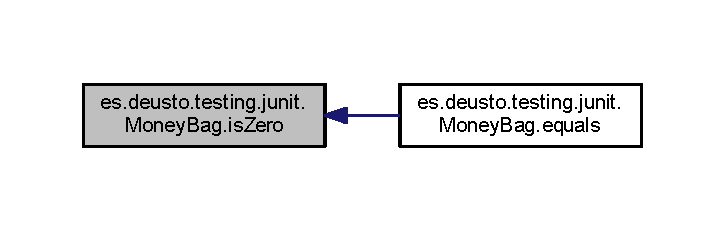
\includegraphics[width=348pt]{classes_1_1deusto_1_1testing_1_1junit_1_1_money_bag_abebc5bc39c3343cb3c4e5fb291fd5893_icgraph}
\end{center}
\end{figure}
\mbox{\Hypertarget{classes_1_1deusto_1_1testing_1_1junit_1_1_money_bag_aa20ce4cc70c2ba0bc9a5ccb96635d506}\label{classes_1_1deusto_1_1testing_1_1junit_1_1_money_bag_aa20ce4cc70c2ba0bc9a5ccb96635d506}} 
\index{es\+::deusto\+::testing\+::junit\+::\+Money\+Bag@{es\+::deusto\+::testing\+::junit\+::\+Money\+Bag}!multiply@{multiply}}
\index{multiply@{multiply}!es\+::deusto\+::testing\+::junit\+::\+Money\+Bag@{es\+::deusto\+::testing\+::junit\+::\+Money\+Bag}}
\subsubsection{\texorpdfstring{multiply()}{multiply()}}
{\footnotesize\ttfamily \mbox{\hyperlink{interfacees_1_1deusto_1_1testing_1_1junit_1_1_i_money}{I\+Money}} es.\+deusto.\+testing.\+junit.\+Money\+Bag.\+multiply (\begin{DoxyParamCaption}\item[{int}]{factor }\end{DoxyParamCaption})}

Multiplies a money by the given factor. 

Implements \mbox{\hyperlink{interfacees_1_1deusto_1_1testing_1_1junit_1_1_i_money_a09154f9713133d4734f72d6a20081209}{es.\+deusto.\+testing.\+junit.\+I\+Money}}.



Definition at line 97 of file Money\+Bag.\+java.

\mbox{\Hypertarget{classes_1_1deusto_1_1testing_1_1junit_1_1_money_bag_abf06bf97e548f95038756608fe0c8351}\label{classes_1_1deusto_1_1testing_1_1junit_1_1_money_bag_abf06bf97e548f95038756608fe0c8351}} 
\index{es\+::deusto\+::testing\+::junit\+::\+Money\+Bag@{es\+::deusto\+::testing\+::junit\+::\+Money\+Bag}!negate@{negate}}
\index{negate@{negate}!es\+::deusto\+::testing\+::junit\+::\+Money\+Bag@{es\+::deusto\+::testing\+::junit\+::\+Money\+Bag}}
\subsubsection{\texorpdfstring{negate()}{negate()}}
{\footnotesize\ttfamily \mbox{\hyperlink{interfacees_1_1deusto_1_1testing_1_1junit_1_1_i_money}{I\+Money}} es.\+deusto.\+testing.\+junit.\+Money\+Bag.\+negate (\begin{DoxyParamCaption}{ }\end{DoxyParamCaption})}

Negates this money. 

Implements \mbox{\hyperlink{interfacees_1_1deusto_1_1testing_1_1junit_1_1_i_money_a741967d7aa89055b6873619303b11385}{es.\+deusto.\+testing.\+junit.\+I\+Money}}.



Definition at line 104 of file Money\+Bag.\+java.

\mbox{\Hypertarget{classes_1_1deusto_1_1testing_1_1junit_1_1_money_bag_a7f1803fe267edca895cdf752b5f46560}\label{classes_1_1deusto_1_1testing_1_1junit_1_1_money_bag_a7f1803fe267edca895cdf752b5f46560}} 
\index{es\+::deusto\+::testing\+::junit\+::\+Money\+Bag@{es\+::deusto\+::testing\+::junit\+::\+Money\+Bag}!subtract@{subtract}}
\index{subtract@{subtract}!es\+::deusto\+::testing\+::junit\+::\+Money\+Bag@{es\+::deusto\+::testing\+::junit\+::\+Money\+Bag}}
\subsubsection{\texorpdfstring{subtract()}{subtract()}}
{\footnotesize\ttfamily \mbox{\hyperlink{interfacees_1_1deusto_1_1testing_1_1junit_1_1_i_money}{I\+Money}} es.\+deusto.\+testing.\+junit.\+Money\+Bag.\+subtract (\begin{DoxyParamCaption}\item[{\mbox{\hyperlink{interfacees_1_1deusto_1_1testing_1_1junit_1_1_i_money}{I\+Money}}}]{m }\end{DoxyParamCaption})}

Subtracts a money from this money. 

Implements \mbox{\hyperlink{interfacees_1_1deusto_1_1testing_1_1junit_1_1_i_money_a1fb4981aa759e3fe0679654bec7a8b61}{es.\+deusto.\+testing.\+junit.\+I\+Money}}.



Definition at line 115 of file Money\+Bag.\+java.

Here is the call graph for this function\+:\nopagebreak
\begin{figure}[H]
\begin{center}
\leavevmode
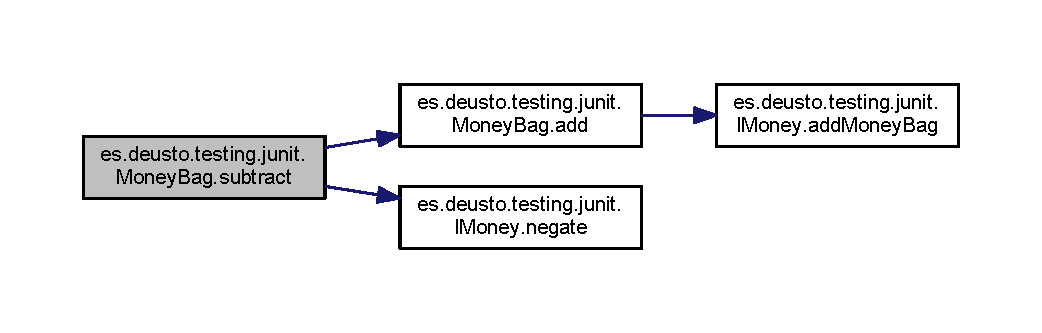
\includegraphics[width=350pt]{classes_1_1deusto_1_1testing_1_1junit_1_1_money_bag_a7f1803fe267edca895cdf752b5f46560_cgraph}
\end{center}
\end{figure}
\mbox{\Hypertarget{classes_1_1deusto_1_1testing_1_1junit_1_1_money_bag_a85b49bdc3ff191abdaa1ad1a065ec5f1}\label{classes_1_1deusto_1_1testing_1_1junit_1_1_money_bag_a85b49bdc3ff191abdaa1ad1a065ec5f1}} 
\index{es\+::deusto\+::testing\+::junit\+::\+Money\+Bag@{es\+::deusto\+::testing\+::junit\+::\+Money\+Bag}!to\+String@{to\+String}}
\index{to\+String@{to\+String}!es\+::deusto\+::testing\+::junit\+::\+Money\+Bag@{es\+::deusto\+::testing\+::junit\+::\+Money\+Bag}}
\subsubsection{\texorpdfstring{to\+String()}{toString()}}
{\footnotesize\ttfamily String es.\+deusto.\+testing.\+junit.\+Money\+Bag.\+to\+String (\begin{DoxyParamCaption}{ }\end{DoxyParamCaption})}



Definition at line 119 of file Money\+Bag.\+java.



The documentation for this class was generated from the following file\+:\begin{DoxyCompactItemize}
\item 
src/main/java/es/deusto/testing/junit/\mbox{\hyperlink{_money_bag_8java}{Money\+Bag.\+java}}\end{DoxyCompactItemize}

\chapter{File Documentation}
\hypertarget{_i_money_8java}{}\section{src/main/java/es/deusto/testing/junit/\+I\+Money.java File Reference}
\label{_i_money_8java}\index{src/main/java/es/deusto/testing/junit/\+I\+Money.\+java@{src/main/java/es/deusto/testing/junit/\+I\+Money.\+java}}
\subsection*{Classes}
\begin{DoxyCompactItemize}
\item 
interface \mbox{\hyperlink{interfacees_1_1deusto_1_1testing_1_1junit_1_1_i_money}{es.\+deusto.\+testing.\+junit.\+I\+Money}}
\end{DoxyCompactItemize}
\subsection*{Packages}
\begin{DoxyCompactItemize}
\item 
package \mbox{\hyperlink{namespacees_1_1deusto_1_1testing_1_1junit}{es.\+deusto.\+testing.\+junit}}
\begin{DoxyCompactList}\small\item\em This is the brief documentation for the Java package \mbox{\hyperlink{namespacees_1_1deusto_1_1testing_1_1junit}{es.\+deusto.\+testing.\+junit}} intended for testing Doxygen. May 12, 2014. \end{DoxyCompactList}\end{DoxyCompactItemize}

\hypertarget{_money_8java}{}\section{src/main/java/es/deusto/testing/junit/\+Money.java File Reference}
\label{_money_8java}\index{src/main/java/es/deusto/testing/junit/\+Money.\+java@{src/main/java/es/deusto/testing/junit/\+Money.\+java}}
\subsection*{Classes}
\begin{DoxyCompactItemize}
\item 
class \mbox{\hyperlink{classes_1_1deusto_1_1testing_1_1junit_1_1_money}{es.\+deusto.\+testing.\+junit.\+Money}}
\end{DoxyCompactItemize}
\subsection*{Packages}
\begin{DoxyCompactItemize}
\item 
package \mbox{\hyperlink{namespacees_1_1deusto_1_1testing_1_1junit}{es.\+deusto.\+testing.\+junit}}
\begin{DoxyCompactList}\small\item\em This is the brief documentation for the Java package \mbox{\hyperlink{namespacees_1_1deusto_1_1testing_1_1junit}{es.\+deusto.\+testing.\+junit}} intended for testing Doxygen. May 12, 2014. \end{DoxyCompactList}\end{DoxyCompactItemize}


\subsection{Detailed Description}
A brief file description testing \mbox{\hyperlink{_money_8java}{Money.\+java}} for file command. May 12, 2014 A more elaborated file description should come here. 
\hypertarget{_money_bag_8java}{}\section{src/main/java/es/deusto/testing/junit/\+Money\+Bag.java File Reference}
\label{_money_bag_8java}\index{src/main/java/es/deusto/testing/junit/\+Money\+Bag.\+java@{src/main/java/es/deusto/testing/junit/\+Money\+Bag.\+java}}
\subsection*{Classes}
\begin{DoxyCompactItemize}
\item 
class \mbox{\hyperlink{classes_1_1deusto_1_1testing_1_1junit_1_1_money_bag}{es.\+deusto.\+testing.\+junit.\+Money\+Bag}}
\end{DoxyCompactItemize}
\subsection*{Packages}
\begin{DoxyCompactItemize}
\item 
package \mbox{\hyperlink{namespacees_1_1deusto_1_1testing_1_1junit}{es.\+deusto.\+testing.\+junit}}
\begin{DoxyCompactList}\small\item\em This is the brief documentation for the Java package \mbox{\hyperlink{namespacees_1_1deusto_1_1testing_1_1junit}{es.\+deusto.\+testing.\+junit}} intended for testing Doxygen. May 12, 2014. \end{DoxyCompactList}\end{DoxyCompactItemize}

%--- End generated contents ---

% Index
\backmatter
\newpage
\phantomsection
\clearemptydoublepage
\addcontentsline{toc}{chapter}{Index}
\printindex

\end{document}
